
% Projekt-Management & Software Engineering
\documentclass[
	11pt,
	DIV=12,
	parskip=half, % Absatzeinstellug 1/2 Zeilenabstand, kein Einzug
	oneside, % Doppeleitiger druck
	final % Entwurf : draft, Endgültig: final
]{scrreprt}

\newcommand{\titleinfo}{Projektmanagement \& Software Engineering - Zusammenfassung}
\newcommand{\authorinfo}{pescara}
\newcommand{\versioninfo}{$Rev: 1.0 $ | 
	gem\"ass Unterricht Michael Trummer/HS2017}

%%%%%%%%%%%%%%%%%%%%%%%%%%%%%%%%%%%%%%%
%% Makros & anderer Low-Level bastel %%
%%%%%%%%%%%%%%%%%%%%%%%%%%%%%%%%%%%%%%%
\makeatletter
%% Makros für Titel, Autor und Datum 
%% Dank diesem Makro stehen Titel, Autor und Datum überall im Dokument zur verfügung
%% Date hat zudem den Default-Wert \today
\def\@Title{}
\def\@Author{}
\def\@Date{\today}
\newcommand{\Title}{\@Title}
\newcommand{\Author}{\@Author}
\newcommand{\Date}{\@Date}
\AtBeginDocument{%
  \let\@Title\@title
  \let\@Author\@author
  \let\@Date\@date
}

%% Makros für den Arraystretch (bei uns meist in Tabellen genutzt, welche Formeln enthalten)
% Default Value
\def\@ArrayStretchDefault{1} % Entspricht der Voreinstellung von Latex

% Setzt einen neuen Wert für den arraystretch
\newcommand{\setArrayStretch}[1]{\renewcommand{\arraystretch}{#1}}

% Setzt den arraystretch zurück auf den default wert
\newcommand{\resetArrayStretch}{\renewcommand{\arraystretch}{\@ArrayStretchDefault}}

% Makro zum setzten des Default arraystretch. Kann nur in der Präambel verwendet werden.
\newcommand{\setDefaultArrayStretch}[1]{%
	\AtBeginDocument{%
		\def\@ArrayStretchDefault{#1}
		\renewcommand{\arraystretch}{#1}
	}
}
\makeatother



\usepackage[automark]{scrpage2} % Header und Footer

 % Load all packages and define styles
\linespread{1.2}
\title{Zusammenfassung}
\author{pescara}

\begin{document}

%\tableofcontents
%\listoffigures
%\listoftables

\clearpage


%%%% Open Tasks %%%
% Input zu Aron, COCOMO, COCOMO II ergänzen
% VL 10, 12, 13, 14 ergänzen


% Kapitel
\pagenumbering{arabic}
\chapter{Libraries \& Frameworks}

\section{Library}
Eine Library (engl. für Bibliothek) stellt bereits implementierte und (getestete) Funktionalitäten (Code) zur Verfügung. Sie enthält statische/konstante Daten und sowie Programmcode. Der Code der Source Files (*.c, *.cpp) werden in die Library gepackt und sind dann nicht mehr sichtbar. Somit müssen nur die Header-Files und Library Files mit dem Executable verlinkt werden. Libraries können über API genutzt werden. Sie ermöglichen den Aufruf von Methoden sowie den Zugriff auf Daten. Es git 2 Arten von Libraries: Static und Shared/Dynamic Libraries. 

\subsection{Static Library}
Library Inhalt wird komplett zur ausführbaren Applikation hinzugefügt. Der Inhalt der Library ist Teil der ausführbaren Applikation. \\
\textbf{ Vorteil:} Library kann nicht vergessen gehen \\
\textbf{Nachteil:} Library wird bei jedem Linken im Speicher abgelegt \\
Typische Dateiendungen: Linux .a / Windows .lib \\

 
\subsection{Shared/Dynamic Libraries}
Shared/Dynamic Libraries werden zur Laufzeit des Programms geladen. Die kann während dem Aufstarten oder irgendwann zur Laufzeit (load/unload) erfolgen. Typischerweise werden die Libraries während dem Aufstarten geladen. Dies bedingt, das die Library schon während dem Linkvorgang bekannt gemacht wird. \textbf{Das Laden der Libraries irgendwann zur Laufzeit (load/unload) wird hier nicht genauer betrachtet.} \\
\textbf{Vorteil:} Library wird nur einmal gespeichert für mehrere Applikationen \\
\textbf{Nachteil:} Applikation kann nicht gestartet werden, falls die Library nicht gefunden wird.
 Typische Dateiendungen: Linux .so (shared object) / Windows .dll (dynamic link library) \\

\section{Framework}
Begriff: engl. framework: Gerüst, Rahmen \\
Ein Framework (engl. für Gerüst, Rahmen) ist gemäss macOS eine Sammlung von Library Versionen. Nebst dem Aufrufen von Methoden (gleich wie  Library) kann ein Framework auch informieren. Es kann auf Ereignisse (Events) registriert werden und gibt so eine Art Skelett vor. Dabei wird das Hollywood Prinzip angewendet (Don't call us, we will call you).
Das Framework beeinflusst somit die Struktur der eigentlichen Anwendung. \\
Bekannte Frameworks: Qt, .Net, EswRobot (Roboter in ProgC Praktika)

\subsection{Library erstellen (-> Prakti 1)}
 
 \adjustbox{width=13cm}{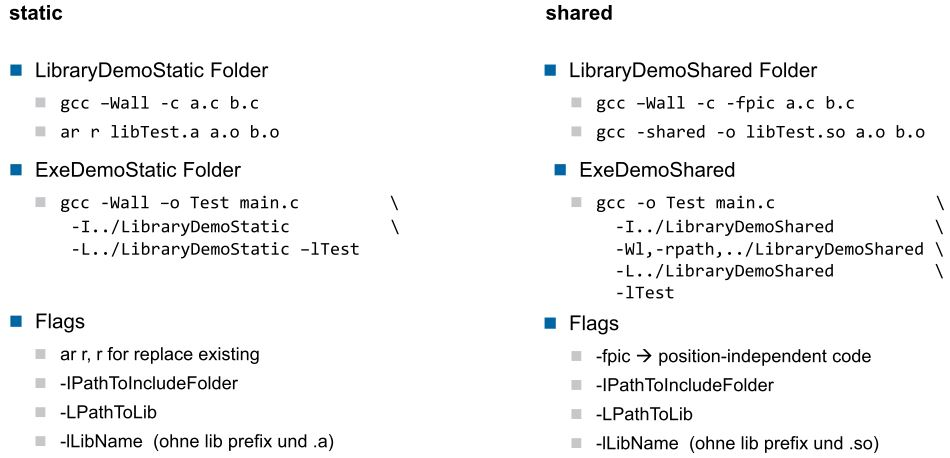
\includegraphics{Figures/createlibrary}}
 
\subsection{Projektstruktur  (-> Prakti 1)}
\textbf{Für Executable} \\
build: Alle object-Files und executable Files (*.o*) \\
libs: Alle nicht System-Libraries (*.a, *.so, *.h) \\
src: Source Code der Applikationen (*.c, *.cpp, *.h) \\

\textbf{Für Libraries} \\
include: Extern verfügbare Header der Library, API (*.h) \\
lib: Library file der zu buildenden library (*.a, *.so) \\
src: Source code der Library inclusive private Header (*.cpp, *.c, *.h)



\chapter{Qt Grundlagen}

\section{Grundlagen}
\textbf{Zweck:} Erstellung von User Interfaces (im speziellen für GUIs) und plattformunabhängige Anwendungen (im Bereich Desktop, Embedded und Mobile) \\
\textbf{Anwendungen:} Skype, Google Earth, Wolfram Research und viele mehr

\subsection{Qt Oberflächen}
\textbf{Qt Desktop (Qt Widgets)} \\
Qt Oberflächen basieren auf der Qt C++ Klassenbibliothek, welche für die GUI-Elemente ("Widgets") entsprechende Klassen wie QLabel, QPushButton etc. bereitstellt. Das GUI wird unter Verwendung dieser Klassenbibliothek als C++-Programm geschrieben und häufig für die Maus- und Tastaturbedienung genutzt. 
\textbf{Neben Qt Widget gibt es noch Qt-Quick (QML) und WebEngine. Der Fokus der Vorlesung liegt auf Qt Desktop.}

\textbf{Qt-Quick} \\
Qt-Quick basiert auf QML (= Qt Meta Language oder Qt Modelling Language), einer speziellen Sprache, welche das Aussehen des Programms festlegt. Verfügt über eine "Deklarative" Festlegung der Darstellung und des Verhaltens, ähnlich wie bei HTML mit Javascript. Qt-Qucik wird vielfach für mobile Applikationen mit Touchscreen Bedienung genutzt.

\textbf{WebEngine} \\
Web Engine wird für die Darstellung von Web Content mit HTML/CSS/JS verwendet. 

\subsubsection{Namenskonventionen}
\begin{itemize}
	\item "Qt" - QtCore - Hauptmodul (wird von allen Modulen genutzt); Weitere Module: QtGui, QtWdigets, QtNetwork, QtSql, QtTest
	\item "Q" - Klasse wie QObject, QApplication, QWidget, QDialog, QString
	\item "q" - globale Variable / Funktionsname wie qApp, qTranslator, qDebug(), qWarning(), qFatal()
	\item "Q\_GROSS" - Qt-Makro-Namen wie Q\_OBJECT, QCOMPARE, QEXPECT\_FAIL, QFETCH
	\item \#include <Qt-Modul- oder Klassenname" wie \#include <QtGui>, \#include <QObject> oder \#include <QString>
\end{itemize}

\section{Meta Object System} 
Dieses System bietet zusätzliche Funktionaitäten zu C++. Es unterstützt das Hollywood Prinizip mittels \textbf{Signals and Slots}. Es basiert auf QObject Klassen, Q\_QBJECT Makro und einem Meta-Object Compiler (moc). 

\subsection{QObject}
Aus der QObject Klasse wurden weitere Qt Klassen abgeleitet wie z.B. QPushBotton, QLabel, QGridLayout, QTimer und QThread. Die QObject Klasse wird zu einem header file hinzugefügt mit \textbf{\#include <QObject>}. QObjects können mit einer Parent-Child-Beziehung verknüpft werden, woraus ein ganzer QObject Tree entstehen kann. Ein Object Tree macht es einfacher eine grosse Anzahl an Dokumente, die miteinander verbunden sind, auf einen Schlag zu löschen. \\
Das Eltern-QObject wird im C'tor des Child-QObjects wie folgt angegeben:\\ 
\textbf{QLabel * child = new QLabel("0000", \&parent);}.\\
Alternativ kann setParent() verwendet werden: \\
\textbf{child->setParent(parent)}
Dies kann jedoch bezüglich der D'tor Reihenfolge problematisch sein (Siehe Prakti 2). \\
Ein Parent-Object kann beliebig viele child-Objects haben, während ein child-Object nur ein parent-Object hat. Die Löschung eines parent objects hat die automatische Löschung sämtlicher child objects zur Folge. Die Löschung eines child objects zerstört einfach die Beziehung zum parent object. 

\subsection{Meta Object Compiler (moc) \& qmake}
Der Meta Object Compiler (moc) durchsucht das header file nach Q\_OBJECT Makros und generiert ein moc\_XXX.cpp File mit dem meta-object relevanten Code erstellt. Diese Dateien müssen bei der Ausführung zur Anwendung hinzugelinkt werden. Für die Verlinkung und Ausführung von Meta Object Compiler (moc), User Interface Compiler (uic) und Resource Compiler (Rcc) wird qmake verwendet, welche diese Qt Compiler automatisch einbindet. Qmake erzeugt aus einer plattformunabhängigen Projektbeschreibung, dem Projektfile (.pro-Datei) ein plattformspezifisches 'makefile'. Diese makefile wird dann von den platformspezifischen Tools wie make dazu verwendet, um die Source-Files zu verarbeiten (compilieren, etc.). Dabei ist qmake selbst ein plattformunabhängiger make-file-Generator. \\Der Befehl lautet: \textbf{qmake <project file name>.pro} 

\begin{figure}[ht]
	\centering
	\adjustbox{width=12cm}{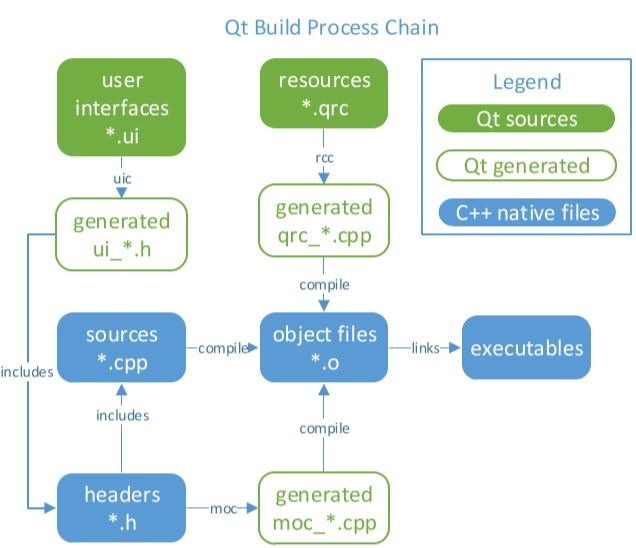
\includegraphics{Figures/qmake}}
\caption[]{Qt Build Prozessablauf}
\end{figure}

\newpage
\subsection{Projektbeschreibung (*.pro)}
\begin{multicols}{2}
\textbf{Keywords:} \\
- QT: Liste von verwendeten Qt Modulen \\
- Target: Name der Applikation (Output File) \\
- TEMPLATE: Projekt Typ: app oder lib \\
- CONFIG: z.B. CONFIG += C++14  \\
- windows/linux/macx: Plattform spezifische   Compilierungsregeln \\
- SOURCES/HEADER/FORMS: Source-, Header- oder Formdateien die dem Projekt hinzugefügt werden sollen \\
\columnbreak
\adjustbox{width=6.5cm}{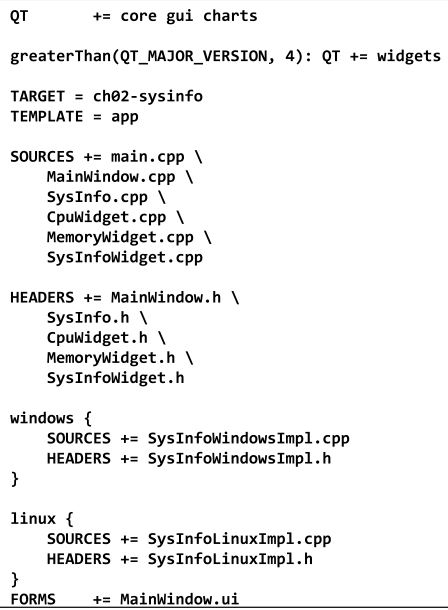
\includegraphics{Figures/keywordspro}}
\end{multicols}


\section{Qt Hallo Welt Beispiel}

\#include <QtWidgets> \\
int main(int argc, char *argv[]) \\
{	QApplication app(argc, argv); \\
	QLabel label ("Hello Qt World!"); \% Erstellen eines Textfelds mit dem Text Hello Qt World! \\
 	label.setAlignment(Qt::AlignCenter); \% Textfeld in der Mitte ausrichten \\
	label.resize(250, 150); \%Breite \& Höhe des Testfelds \\
	label.setWindowTitle("My first Qt‐Program"); \%Titel des Popup Fenster  \\
	label.show(); \%Befehl zum Anzeigen des Textfelds \\
	return app.exec(); } 

\subsection{QApplication Klasse}
Die QApplication Klasse ist pro Qt Applikation nur einmal vorhanden. Sie ist zuständig für das Event handling und weitere Qt Framework spezifische Funktionälitäten. Eine der Methoden heisst exec(). In dieser Methode verbirgt sich die while(1) Schleife.
QApplication Klasse ist zudem für die Initialisierung der Applikation mit optionalen Funktionen wie beispielsweise font() und doubleClickInterval() zuständig. 


\chapter{QWidgets \& Layout}

\section{QWidgets}
Applikation mit GUI = Problem-Domain + Darstellung + Interaktion \\
Bsp.: Counter = Funktionalität (inkrementieren und dekrementieren) + Fenster mit inc \& dec Buttons und der Anzeige des aktuellen Counter-Stands + Inkrementieren, wenn inc-Button gedrückt.
\textbf{Allgemeine Konzepte von GUI Frameworks} \\
\textbf{Ansicht festlegen:} Visuelle Elemente in der Benutzeroberfläche werden mittels Klassen vom GUI Framework zur Verfügung gestellt. \\
\textbf{Interaktion} mit dem Programmbenutzer -> Signals \& Slots

\subsection{QWidget Klasse}
QWidget (Widget = "Window Gadget") ist eine Basisklasse für alle anderen Qt Widgets wie bspw. QLabel, QLineEdit, QPushButton
QWidget übernimmt als Parent-Widget folgende Aufgaben:
- Anzeigen, verstecken, freigeben, sperren -> wird auch auf die Child-Widgets angewendet \\
- Weiterleiten von Ereignissen an die betroffenen Child-Widgets\\
- Memory Management \\
\begin{figure}[hb]
	\centering
\adjustbox{width=7.5cm}{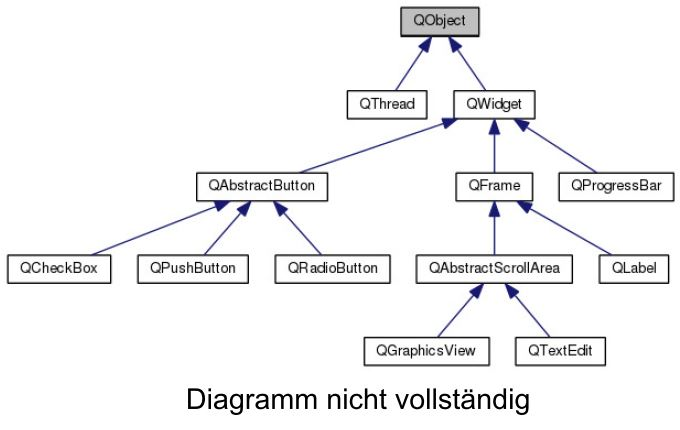
\includegraphics{Figures/qtwidgets_objekte}}
	\caption[]{Qt Vererbungen von QObject und QWidget}
\end{figure}

\section{Layout}

\begin{tabular}{|l|l|l|}
	Art & Selbst codiertes GUI & GUI-Designer (Qt Creator) \\
	Beschreibung & C++ Code für GUI Beschreibung & Interaktives Tool \\
	Vorteil & kann sich zur Laufzeit ändern & schnell zusammen "geklickt" \\
	Nachteil & aufwändig, Code selber schreiben & Nur statische Design möglich
\end{tabular}

Bei der Erstellung eines GUIs mittels WYSIWYG Editor – GUI-Designers (Qt-Creator) erfolgt die Anordnung der Widgets innerhalb eines sogenannten Formulars mit Hilfe eines interaktiven Tools. Es erfolgt eine automatische Umwandlung der Formulardaten (*.ui) in entsprechenden Programmcode mittels uic. 

\subsection{Manuelles Layout}

\begin{figure}[ht]
	\centering
	\adjustbox{width=0.8\textwidth}{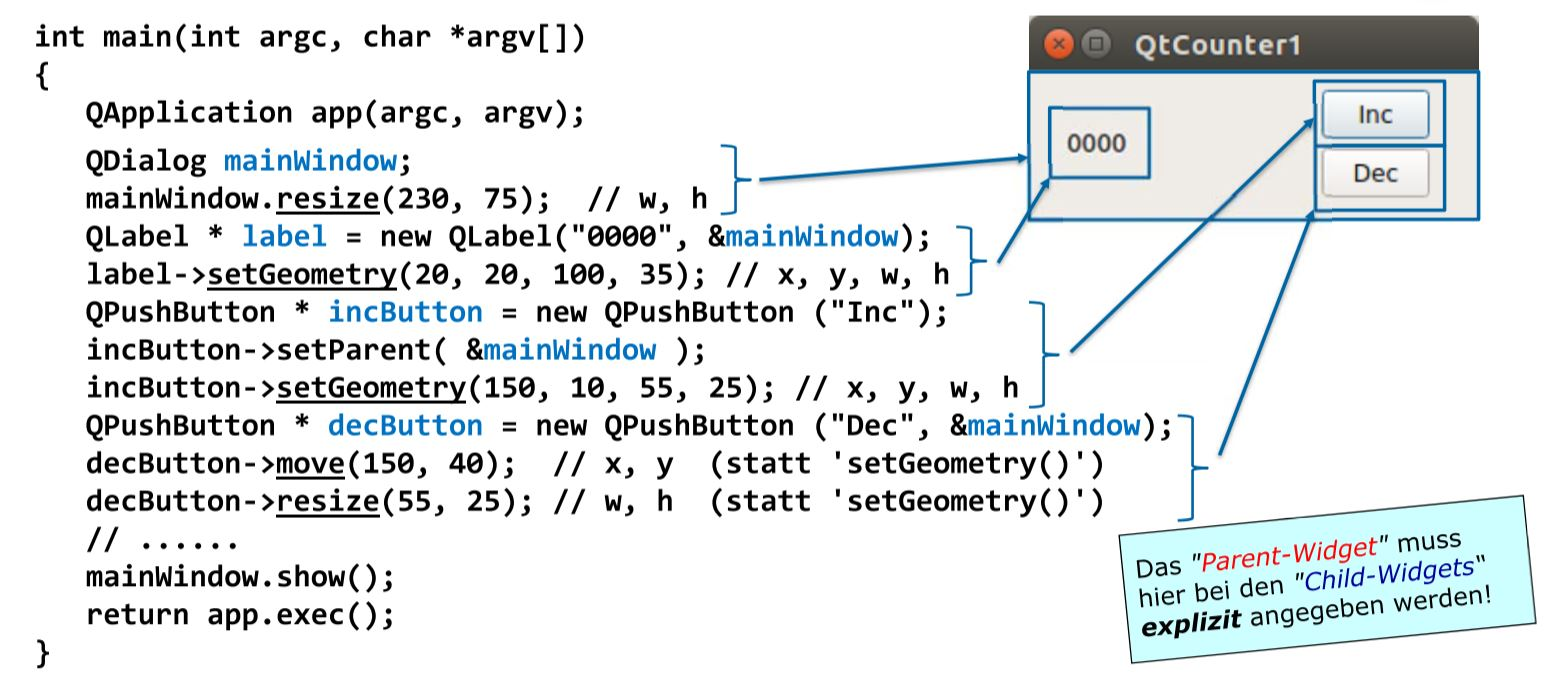
\includegraphics{Figures/Layout}}
	\caption[]{Beispeil eines manuellen Layouts}
\end{figure}

Die Positionierung erfolgt mittels eines Koordinatensystems bei dem der Ursprung (0,0) in der linken oberen Ecke ist. Die Position und Grösse wird in Pixel angegeben. Die x-Werte erhöhen sich nach rechts, während die y-Werte nach unten ansteigen. (x, y) sind die Koordinaten der linken oberen Ecke eines Widgets innerhalb eines anderen, des äusseren Widgets. w, h sind Breite und Höhe des inneren Widgets.

Methoden zur Festlegung von Position und/oder Grösse
\textbf{void QWidget::setGeometry(int x, int y, int w, int h);} \\
\textbf{void QWidget::resize (int w, int h);} \\
\textbf{void QWidget::setFixedSize(int width, int height);} \\
\textbf{void QWidget::move (int x, int y);} \\

\section{Qt Layout Manager}
\begin{figure}[ht]
	\centering
	\adjustbox{width=0.7\textwidth}{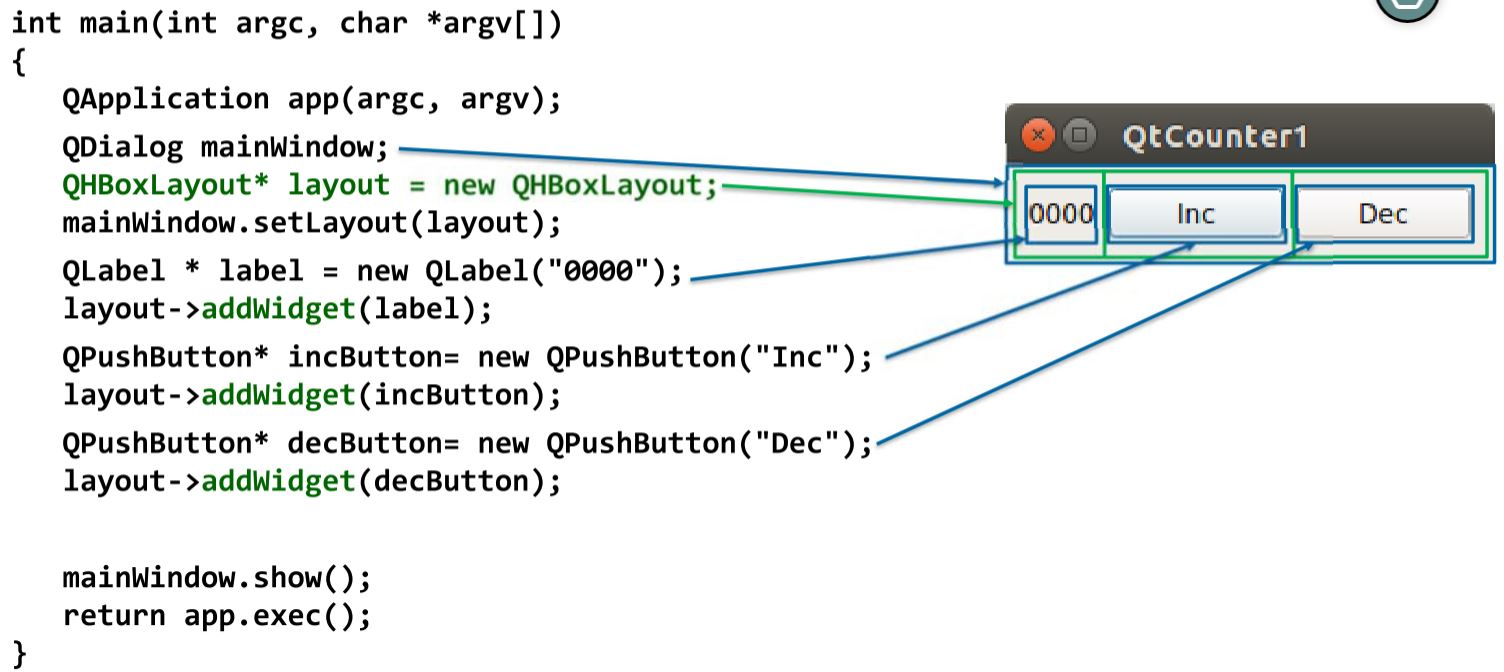
\includegraphics{Figures/QtLayoutManager}}
	\caption[]{Qt Layout Manager}
\end{figure}

Klassen, welche von QLayout ableiten: \\
- QHBoxLayout: Ordnet Elemente horizontal  an \\
- QVBoxLayout: Ordnet Elemente vertikal an \\
- QGridLayout: Ordnet Elemente in einem zweidimensionalen Gitters an. \\
- QFormLayout: Ordnet Elemente in Form von Zeilen an Zeile = QLabel gefolgt von anderem QWidget (z.B. QLineEdit) \\
- QStackedLayout: "Aufeinandergelegte" Widgets (Stapel), nur immer ein Widget ist sichtbar \\
 

Das QLayout-Objekt ist bei einem Parent-Widget zuständig für das Layout (Anordnung) von dessen Child-Widgets:  \\
\textbf{QDialog mainWindow;} \\
\textbf{QVBoxLayout* mainLayout = new QVBoxLayout;} \\
\textbf{mainWindow.setLayout(mainLayout);}
Wird ein child-widget mit addWidget(label) hinzugefügt, dann wird es automatisch mit dem parent Widget verknüpft. 
Das QLayout-Objekt ist selbst ein "Kind" vom "Parent-Widget". Es ist zweckmässig, sich das QLayout-Objekt als ein spezielles Geschwister vorzustellen, das als Kindermädchen ("Nanny") der "Child-Widgets" wirkt. QLayout-Objekte haben nie QWidget-Objekte als eigene Kinder.

Das QLayout-Objekt informiert das "Parent-Widget" automatisch über die Existenz der "Child-Widgets". Das geschieht mittels der addWidget Methode des Layout Managers: \\
\textbf{QLabel * label = new QLabel("0000");}
\textbf{mainLayout‐>addWidget(label);}
Das "Parent-Widget" muss bei den "Child-Widgets" nicht explizit angegeben werden! \\
Layouts können auch verschachtelt werden:
\textbf{QVBoxLayout* mainLayout = new QVBoxLayout;}
\textbf{QHBoxLayout* bottomLayout = new QHBoxLayout;}
\textbf{mainLayout‐>addLayout(bottomLayout);}

\section{Qt Layout Manager}
\begin{figure}[ht]
	\centering
	\adjustbox{width=0.7\textwidth}{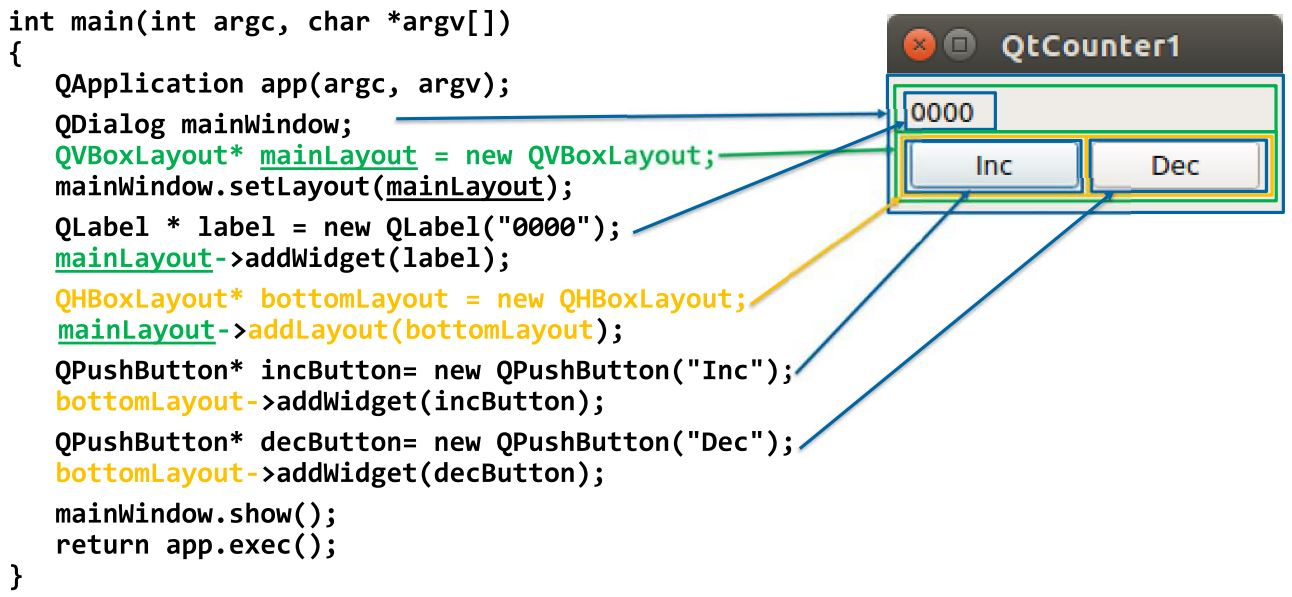
\includegraphics{Figures/layoutmitverschachtelung}}
	\caption[]{Qt Layout: Beispiel mit Verschachtelung}
\end{figure}

\subsection{GUI Erstellung mittels Qt-Creator}

Der Zugriff auf die Widgets:
Widget::Widget(QWidget *parent) :
QWidget(parent),
\textbf{ui(new Ui::Widget)} -> Erstellt ein Layout
{
\textbf{	ui‐>setupUi(this);}
\textbf{	ui‐>lineEdit‐>setText("Test");} -> Setzt den Text in lineEdit Widget
}
Widget::~Widget()
{
\textbf{delete ui;} -> Löscht das Layout
}

ui->lineEdit->setText("Test");

\subsection{Top-Level-Window/Widget}
Definition: Widgets auf der obersten Hierarchiestufe des Widget-Trees.  Widgets ohne Eltern \\
Jedes Widget kann ein "Top-Level-Window" sein
Der Titelbalken ("TitleBar") gehört nicht zu Qt (!), sondern wird vom Betriebssystem erzeugt.
Übliche Widgets für "Top-Level-Windows/Widget":

\textbf{QMainWindow}: Typisch als Applikations-Window (Hauptfenster). Es hat Toolbars und eine Statusbar.

\textbf{QDialog "Popup-Window"}: typisch für Abfragen wie "Soll dies Datei wirklich gelöscht werden?" "Okay", "Abbrechen". \\
Häufig modal, d.h. die Hauptanwendung bleibt blockiert, bis der Dialog beendet ist. Die Standarddialog-Klasse von Qt ist QMessageBox
\textbf{QWidget}: Einfaches Fenster, üblicherweise "non-modal" (d.h nicht blockierend). In den weiteren Beispielen wird meistens QWidget als Top-Level Widget verwendet


\newpage
\section{Qt Widget Collection für Darstellungen (Selbststudium)}


\begin{minipage}{5cm}
	\small{	Single Page Container}
\end{minipage}
\begin{minipage}{5cm}
	\small{Multi Page Container}
\end{minipage}
\begin{minipage}{5cm}
	\small{Button widgets}
\end{minipage}

	\adjustbox{width=5cm}{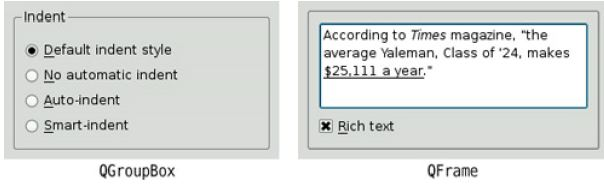
\includegraphics{Figures/scontainer}}
	\adjustbox{width=5cm}{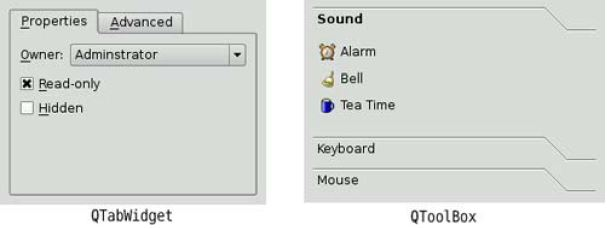
\includegraphics{Figures/mcontainer}} 
	\adjustbox{width=5cm}{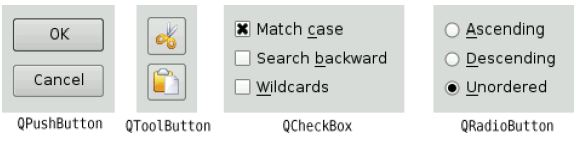
\includegraphics{Figures/buttonwidgets}}
	\\

\begin{minipage}{10cm}
	\small{Input Widget}
\end{minipage}
\begin{minipage}{5cm}
	\small{Color and Font Dialog}
\end{minipage}

	\adjustbox{width=5cm}{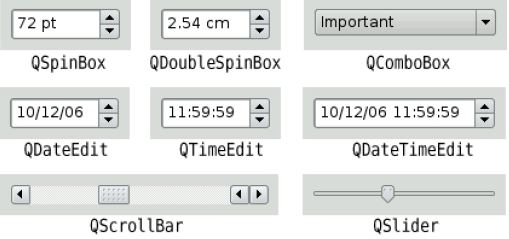
\includegraphics{Figures/inputwidget}}
	\adjustbox{width=5cm}{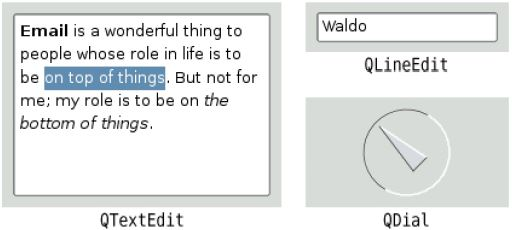
\includegraphics{Figures/inputwidget2}}
	\adjustbox{width=5cm}{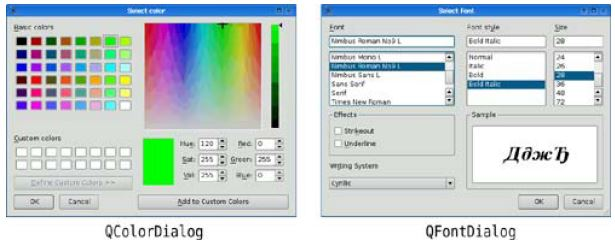
\includegraphics{Figures/cwidget}} \\
	
\begin{minipage}{8cm}
	\small{Item View Widgets}
\end{minipage}
\begin{minipage}{8cm}
	\small{Display Widgets}
\end{minipage}	
	
	\adjustbox{width=8cm}{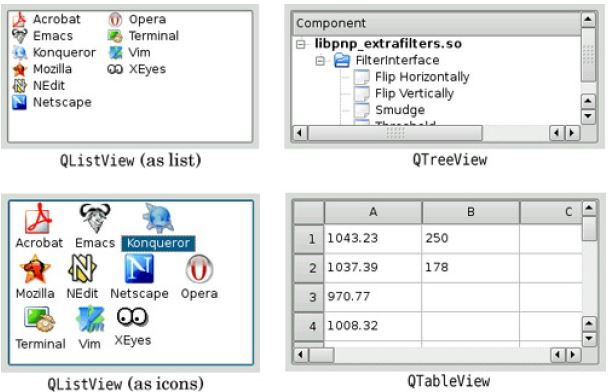
\includegraphics{Figures/vwidget}}
	\adjustbox{width=8cm}{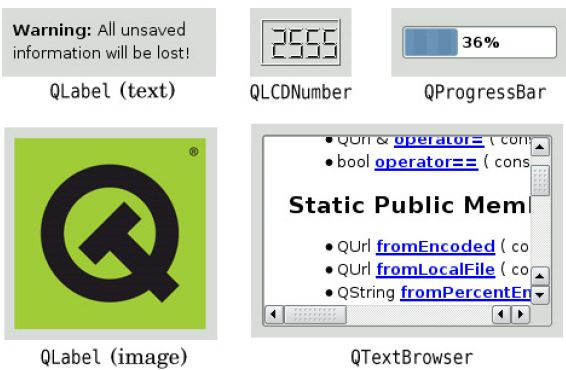
\includegraphics{Figures/dwidget}} \\
	
	\begin{minipage}{8cm}
		\small{File und Print Dialogs}
	\end{minipage}
	\begin{minipage}{8cm}
		\small{Feedback Dialogs}
	\end{minipage}	
	
	\adjustbox{width=8cm}{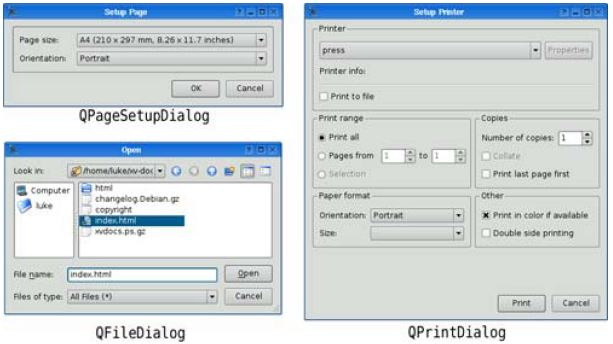
\includegraphics{Figures/pwidget}}
	\adjustbox{width=8cm}{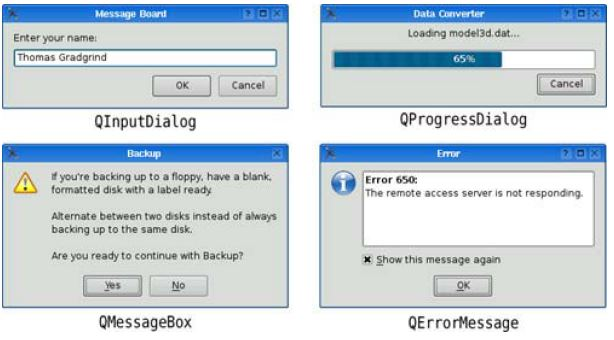
\includegraphics{Figures/fwidget}}


\chapter{Callback \& Signals und Slots - Interaktion}

\section{Reaktive Systeme}

Reaktive Systeme (reactive systems) reagieren auf (oft externe) Ereignisse wie digitale Inputs, die Erreichung von analogen Schwellenwerten, Timer, Buttonclicks oder ähnliches in GUI, etc. Dabei bestehen häufig auch Echtzeitanforderung an das System. Embedded Systems sind häufig auch reaktive Systeme. 
Ereignisse sind per Definition asynchron, d.h. sie treten zu einem beliebigen Zeitpunkt ein, während ein "normales" Programm immer synchron (zuerst das, dann das, dann …) ist. 

\subsection{Pooling}
Ereignisse können von synchronen Programmen durch Polling verarbeitet werden, d.h. das 
Programm fragt periodisch oder dauernd ab, ob irgendein Ereignis eingetreten ist. Polling ist sehr einfach zu implementieren. 
Dabei entstehen jedoch üblicherweise sehr viele Leerabfragen, d.h. bei vielen Abfragen ist nichts eingetreten, was eine unnötige Prozessorbelastung bewirkt. Sie können durch periodische Abfragen (Kopplung an Timer) reduziert aber nicht vermieden werden.
Die maximale Reaktionszeit wird durch die Abfrageperiode und die Anzahl Abfragen (Stichwort: Looptime bei SPS) definiert. 

\subsection{C Callbacks}
Callbacks stellen bidirektionale Verbindungen von Modulen mit C dar. 

\textbf{Beispiel einer bidirektionalen Verbindung zwischen A und B} \\
 Dabei kennt Klasse A, B UND Klasse B kennt ebenfalls die Funktion von Klasse A.
C-File von A: \\
void aInit(void) \\ \{
	bRegisterFoo(\&aFooY);  \textbackslash*Eine Funktion von B wird in A aufgerufen. Der Parameter der Funktion ist eine Funktion der Klasse A. /* 
\}\\
void aFooY(void) \\ \{ 
	printf("aFooY called\textbackslash n");
\}

C-File von B: \\
static void (*regFct)(void); \% Funktionspointer \\
void bFooX(void) \\
\{ 
	if (0 != regFct)\\
	regFct();
\}\\
void bRegisterFoo(void (*fct)(void))\\
\{
	regFct = fct; \textbackslash* Die von der Klasse A aufgerufene Funktion bRegisterFoo hat als Parameter eine Funktion aus der Klasse A, welche dem Funktionspointer regFct zugewiesen wird und wieder auf die Funktion aFooY in der Klasse A zeigt. /*
\}



\textbf{Beispiel einer unidirektionalen Verbindung zwischen Klasse A und B} \\
Dabei hat die Klasse A eine Verbindung zu Klasse B, aber nicht umgekehrt. 

Das File der Kasse A sieht folgendermassen aus: \\
\textbf{\#include "B.h"  \% Das Header File von B wird eingefügt}
class A \\
{ public: \\
	\textbf{A() { b.foo();	}  \% Verknüpfung mit B}\\
	void fooY() {} \\
	private: \\
	\textbf{B b; \% Ein Objekt der Klasse B kann somit in A aufgerufen werden} \\
};

\textbf{Bidirektionale Verbindung von Klassen} \\
Klasse A kennt Klasse B UND Klasse B kennt Klasse A -> Das funktioniert so nicht, da es sich um ein circular include handelt. Eine Ausnahme stellt ein Class Forwarding dar. \\
\begin{figure}[ht]
	\adjustbox{width=9cm}{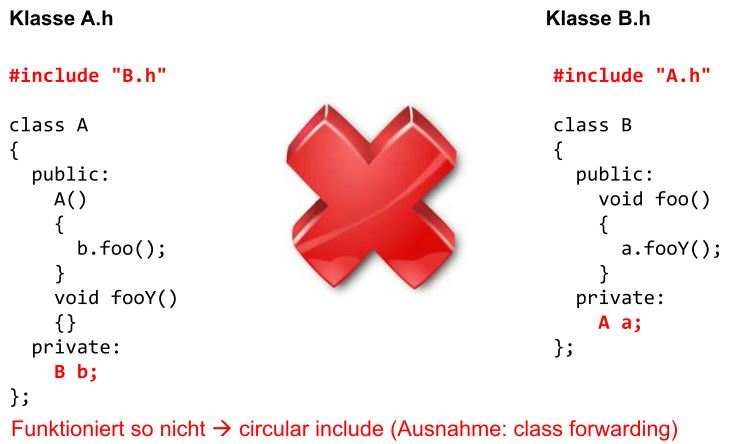
\includegraphics{Figures/bidirektional}}
	\caption[]{Keine gültige Bidirektionale Verbindungen von A und B}
\end{figure}

Die nachfolgenden Versionen einer bidirektionalen Verbindung: \\
V1:Klasse A kennt Klasse B UND Klasse B kennt Objekt von Klasse A
Funktioniert, da in Header-File B.h nur Pointer auf A, der Rest ist im B.cpp File. Unschön: B muss immer noch A kennen (class forwarding erforderlich). Besser: A sollte unabhängig von B sein

V2:Klasse A kennt Klasse B UND Klasse B kennt Objekt von Klasse C, Klasse A ist eine Klasse C. Bessere Variante als V1: B kennt nicht mehr A direkt

V3:Klasse A kennt Klasse B UND Klasse B kennt Objekt von Klasse C, Klasse A ist eine Klasse C. Besser Variante als V2: der Funktionspointer wird weggelassen, da überflüssig

\begin{figure}[ht]
\adjustbox{width=12cm}{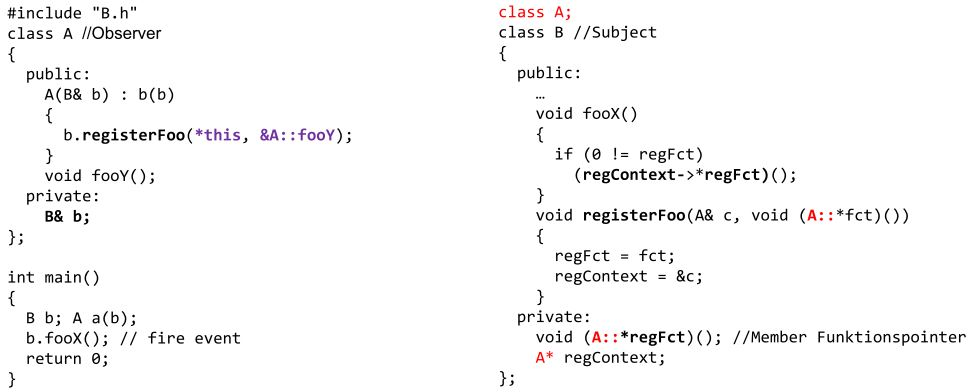
\includegraphics{Figures/bidirektionalv1}}
\adjustbox{width=12cm}{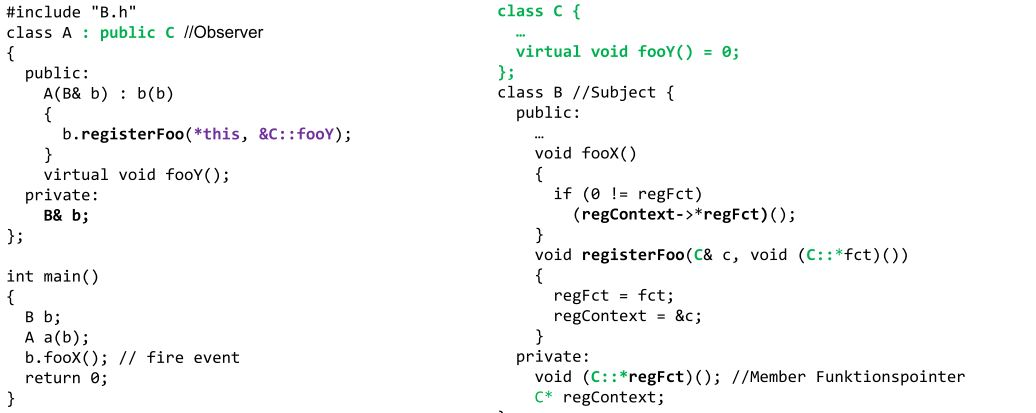
\includegraphics{Figures/bidirektionalv2}}
\adjustbox{width=12cm}{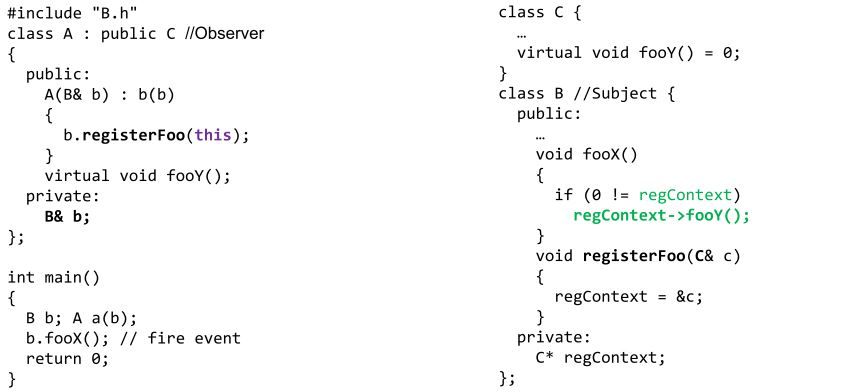
\includegraphics{Figures/bidirektionalv3}}
\caption[]{Bidirektionale Verbindungen: V1-V3}
\end{figure}

Abstraktere C++ Umsetzungen folgen im Modul OOAD: Observer Pattern. 
Die kennengelernten Callback und Observer Methoden können für native C++ verwendet werden. In Qt können Signal/Slots verwendet werden.

\section{Qt Signals and Slots: Qt Interaktion zwischen QObjects}

Qt verwendet anstatt Callbacks ein Signal-Slot Prinzip. Analogie zu Callbacks: Das zu informierende Objekt (Observer) hat einen slot, Das informierende Objekte (Subject) hat ein signal, die Registrierung erfolgt über eine connect Funktion. 

Es wird der Funktionspointer von C++-Member verwendet. Signals und Slots werden mit dem QObject::connect() verbunden. \\ 
Form: connect(SenderObj* (=Subject), SenderMethode* (signal1), EmpfängerObj* (= Observer), EmpfängerMethode* (slot2)) \\
Bsp.: connect(\&b, \&B::fooX, \&a, \&A::fooY);

Beispiel: 
\begin{figure}[ht]
	\centering
	\adjustbox{width=0.9\textwidth}{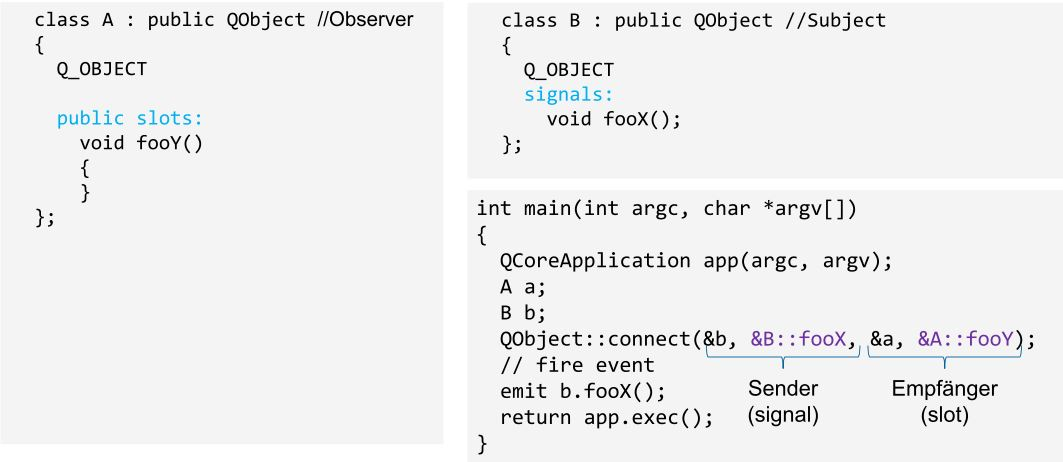
\includegraphics{Figures/bspsignal}}
	\caption[]{Beispiel Signal \& Slots}
\end{figure}

%\begin{figure}[ht]
%	\centering
%	\adjustbox{width=0.9\textwidth}{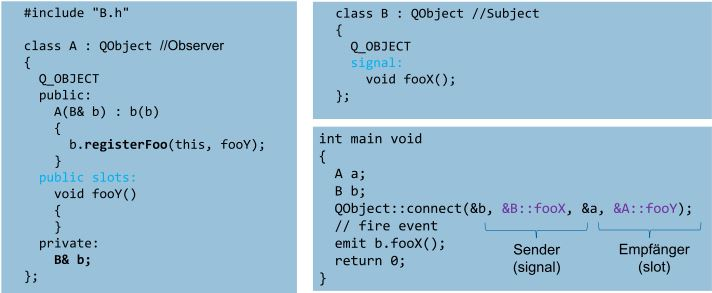
\includegraphics{Figures/bspsigslot}}
%	\caption[]{Beispiel Signal \& Slots}
%\end{figure}

\subsection{Signals - Signal-Memberfunktion}
Signals werden nur deklariert und nicht implementiert. Es werden keine Zugriffsrechte wie private public oder protect verwendet. Der Rückgabetyp ist immer void. Ein Signalaufruf erfolgt mit \textbf{emit method(value)}. Die C++ Definition erfolgt mit \textbf{\#define signals public}. Ein Signal kann mit mehreren Slots oder anderen Signalen verbunden werden. Mehrere Signal können mit demselben Slot verbunden werden. Es kann einen Übergabeparameter haben.

\subsection{Slots}
Slots sind immer public (by default). Für private slots muss das Keyword slots weggelassen werden. Die C++ Definition lautet \textbf{\#define slots}. Slots können einen Übergabeparameter haben. 

\subsection{Signals \& Slots: Connect}

Der Parameter Typ und Anzahl muss stimmen
Signal: Slot:
void clicked() -> void onClicked()
void indexChanged(int idx) -> void onIndexChanged(int idx)


\textbf{Ab Qt5 - mit Funktionspointer} \\
connect(senderObj, \&SenderClass::senderMethod \\
revObj, \&RevClass:revMethod); \\
+ weniger Klammern  \\
+ keine Datentypen für Parameter; aber Compiler meldet Fehler

\textbf{Alte Notation} \\
connect(button, SIGNAL(clicked()) \\
count, SLOT(incValue())); \\
Keine Compilerfehlermeldungen, falls falsch -> wird zur Laufzeit geprüft

\textbf{Globale Funktionen als Slots (ab Qt5)} \\
void printValue(int x) \\
\{ 	std::count << "Value=" << x << std::endl;\} \\
connect(button, \&QPushButton::clicked, \&printValue); 


\textbf{Überladene Methoden} \\
void QLabel::setNum(int num) \\
void QLabel::setNum(double num) \\
connect(…, static\_cast<void (QLabel::*)(int)>(\&QLabel::setNum), …, …);

\begin{figure}[ht]
	\centering
	\adjustbox{width=0.7\textwidth}{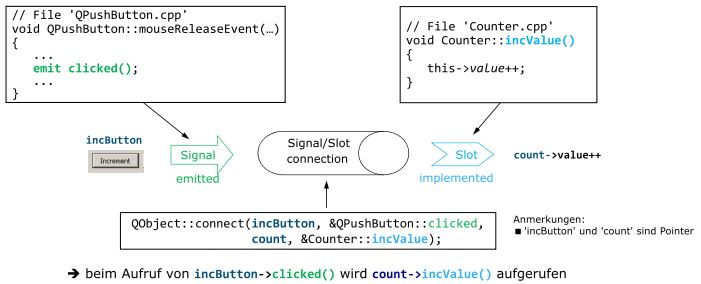
\includegraphics{Figures/sigausframework}}
	\caption[]{Beispiel mit Signal aus Framework}
\end{figure}

\begin{figure}[ht]
	\centering
	\adjustbox{width=0.7\textwidth}{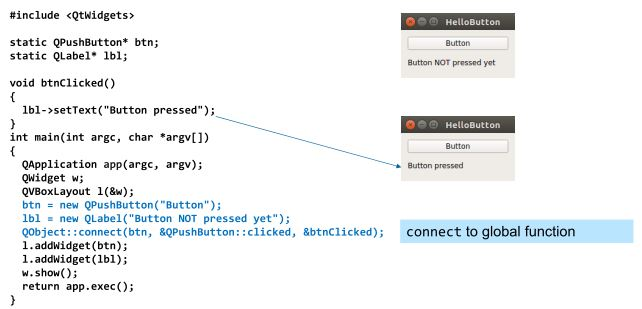
\includegraphics{Figures/hellobutton}}
	\caption[]{"Hello Button" - GUI Programm}
\end{figure}

\begin{figure}[ht]
	\centering
	\adjustbox{width=9cm}{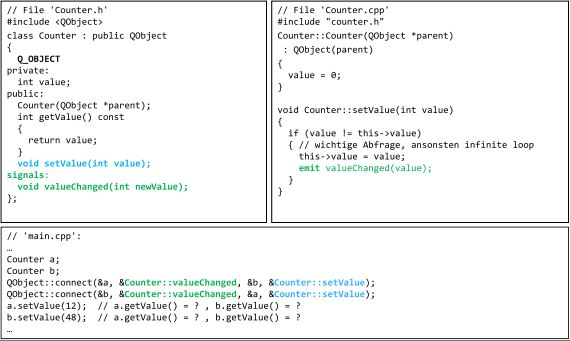
\includegraphics{Figures/selfconnect}}
	\caption[]{Counter Beispiel: Connect mit sich selbst}
\end{figure}



\chapter{Projekt Management}

\section{Management von Softwareprojekten}

Eine \textbf{Organisation} kann definiert werden über ihre Struktur, ihre Funktion oder die Institution, welche sie darstellt.

Das \textbf{Management} übernimmt Leitungsaufgaben in Projekten und Unternehmen. Es handelt sich um eine Gruppe von Personen welche sich mit typischen Aufgaben wie Planung, Delegation, Organisation sowie Führung und Erfolgskontrolle. 

Ein \textbf{Artefakt} ist ein primäres oder sekundäres Arbeitsergebnis, welches durch Projektaktivitäten erstellt wird. Beispiele: Pflichtenheft, Architekturentwurf, Testfallbeschreibung. 

Ein \textbf{Projekt} ist komplex, neuartig, zeitlich befristet und weist begrenzte Ressourcen / Budget, Teamarbeit und messbare Ziele und Ergebnisse auf. Projektbeispiele sind ein neu entwickeltes, lauffähiges Softwaresystem, Teilergebnisse für die Entwicklung von Software, die Migration einer Software auf eine andere 
Hardwareplattform. 
Keine Projekte sind Routinetätigkeiten, Vorhaben des "daily business" wie beispielsweise Archivverwaltung und Kantinenbewirtschaftung. 
Ein Grenzbereich könnte die Pflege der Datenverarbeitung darstellen. 

Softwareentwicklungsprojekte unterscheiden sich nicht grundlegend zu anderen Entwicklungsprojekten wie Elektrotechnische Erzeugnisse, Maschinen und Bauwerke. Es gibt jedoch einige signifikante Unterschiede durch die \textbf{Immaterialität} (Abstraktes Artefakt, bei SW nur Entwicklungsprozesse und 
Inbetriebnahme und keinen wirklichen Produktions- bzw. Fertigungsprozess). Die Folge davon ist, dass Fehler bei materiellen Produkten in der Regel noch während Planung oder Durchführung der Fertigung erkannt werden. 

Projektstatistiken \\
Gemäss der CHAOS 2004 Umfrage kam es 2005 zu 15.52 \% und 2007 zu 11.54 \% Projektabbrüchen. Die Statistiken zeigen einen Trend, sollten jedoch nicht absolut verglichen werden. Gemäss der Standish Group sind die Zahlen nicht glaubhaft («Nur weil jemand eine Frage stellt, bedeutet das nicht, 
dass wir antworten. Tatsächlich antworten wir 
eher nicht»)

Gescheiterte Software Projekte \\
Der Ariane 5 Fehlstart
Am 4. Juni 1996 startete die Ariane 5 Rakete zu ihrem Erstflug. Nach genau 36,7 Sekunden sprengte sich die Rakete selbst inklusive vier Satelliten. \\Kosten: 500 Mio Dollar \\
Ursache: 64Bit zu 16Bit-Wandlung

\subsection{Ziele des Managements}
Die Ziele des Software Engineering sind ein Produkt kostengünstig, termingerecht und in angemessener Qualität anzuliefern. Teilziele sind die Beherrschung von Zeit und Kosten. Kann ein unterschiedlicher Fokus gelegt werden: kostenfixiert, terminfixiert, leistungsfixiert, mit dem Ziel der Erreichung von Qualitätszielen, der Sicherung von Investitionen oder der Einhaltung von Rahmenbedingungen. 

Folgender Zusammenhang gilt zwischen den Fehlerkosten von Softwareprojekten:
\begin{figure}[hb]
	\centering
	\adjustbox{width=10cm}{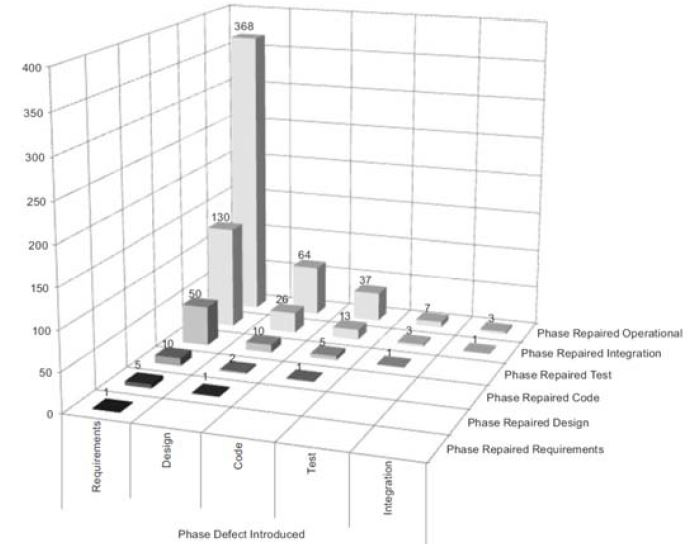
\includegraphics{Figures/bugfixingcost}}
\caption[]{Relative Bugfixing Kosten}
\end{figure}
	
\textbf{Faktoren für erfolgreiche Projekte sind:} \\
- Angestellte: Hohe Motivation der Mitarbeiter / Erfahrene \\ Projektmanager und Entwickler \\
- Kundenorientierung \\
- Management: Klare Projektziele / Realistische Projektpläne / Klare Verantwortungsstrukturen / Offene Kommunikationskultur \\
- Prozessorientierung \\
- Dokumentation und Artefakte \\
- Modularisierung und Wiederverwendung



\section{Produkt-, Projekt- und Softwarelebenszyklus}
Der Softwarelebenszyklus ist als Spezialisierung des Produktlebenszyklus anzusehen. 
\begin{figure}[ht]
	\centering
	\adjustbox{width=11cm}{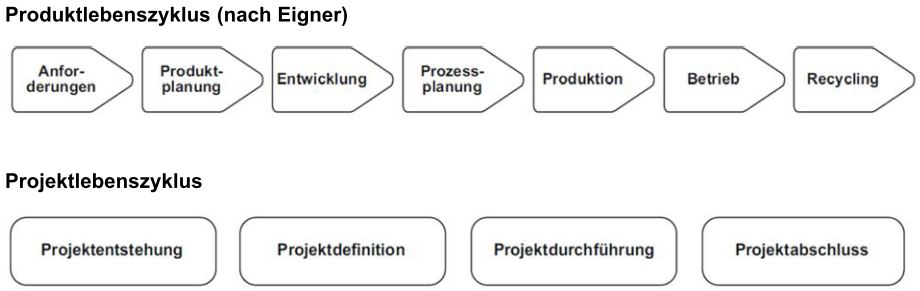
\includegraphics{Figures/lebenszyklus}}
	\caption[]{Produkt- \& Projektlebenszyklus}
\end{figure}


\subsection{Softwarelebenszyklus}
\begin{itemize}
	\item Analyse: Anforderungsfestlegung
	\item Design: Grob- \& Feinentwurf (Architektur, Programmstruktur)
	\item Implementierung
	\item Test und Integration
	\item Betrieb \& Wartung: Erprobung und Inbetriebnahme sowie Wartung und Weiterentwicklung
	\item Ausserbetriebnahme
\end{itemize}
Der Softwarelebenszyklus muss nicht sequentiell ablaufen. Zudem kann der Prozess iterativ mehrmals durchlaufen werden. 

\subsection{Phasen im Projektlebenszyklus}
\begin{itemize}
	\item Projektentstehung
	\begin{enumerate}
		\item Projektidee entwickeln: Ziele, Bedarf, Chancen festlegen \& ggf. Projektvorstudie durchführen -->
		\textbf{M1: Projektskizze} 
		\item Aufwand schätzen sowie Anforderungen und Ziele grob festlegen: Anforderungen notieren, grober Plan definieren, Schätzung durchführen und in einem Business Case zusammenfassen -->
		\textbf{M2: Projektauftrag}
		\item Angebots- und Vertragswesen: Lastenheft und Angebot festlegen und Gegenpartei übergeben -->
		\textbf{M3: Vertrag / Projektvereinbarung}
	\end{enumerate}
	\item Projektdefinition
	\begin{enumerate}
		\item Projekt strukturieren und Projektteam organisieren
		\item Definition eines Projektmanagementverfahrens und Erstellen eines Projekthandbuchs
		\item Definition eines QS-Verfahrens und Erstellen eines QS-Handbuch
		\item Aufbau einer Projektinfrastruktur
		\item Projekt planen bzw. Erstellen eines Projektplan
	\end{enumerate}
	\item Projektdurchführung \\
	Durchführung eines iterativen Entwicklungsprozess gemäss den Phasen des V-Modells. Der Input entspricht dem Pflichtenheft und die Lieferung dem Output. Zeitgleich werden die iterativen Phasen von Planung (Soll-Vorhaben) -->Kontrolle  (Messung von Kennzahlen und Soll-/Ist-Vergleich) -->Steuerung (Steuerungsmasssnahmen hinsichtlich QS oder Projektmanagement) --> Anpassung des Vorhabens durchlaufen. 
	\begin{itemize}
		\item Erfassung und Verfeinerung der Anforderungen
		\item Systementwurf
		\item Implementierung, Verifikation und Test
		\item Test und Integration
		\item Erprobung und Übergabe
	\end{itemize}
	\item Projektabschluss \\
	\begin{enumerate}
		\item Ergebnisse der Entwicklung: Code, Systemarchitektur, Tests, Dokumentation, System
		\item Lieferung abnehmen und System in Betrieb setzen (inkl. Freigaben)
		\item Projekt abschliessen beinhaltet die Sicherung der gemachten Erfahrungen, die Auflösung des Projektteams und die Projektabrechnung --> Projektabschlussbericht
	\end{enumerate}
\end{itemize}
Mx: stehen für die erreichten Meilensteine innerhalb einer Phase

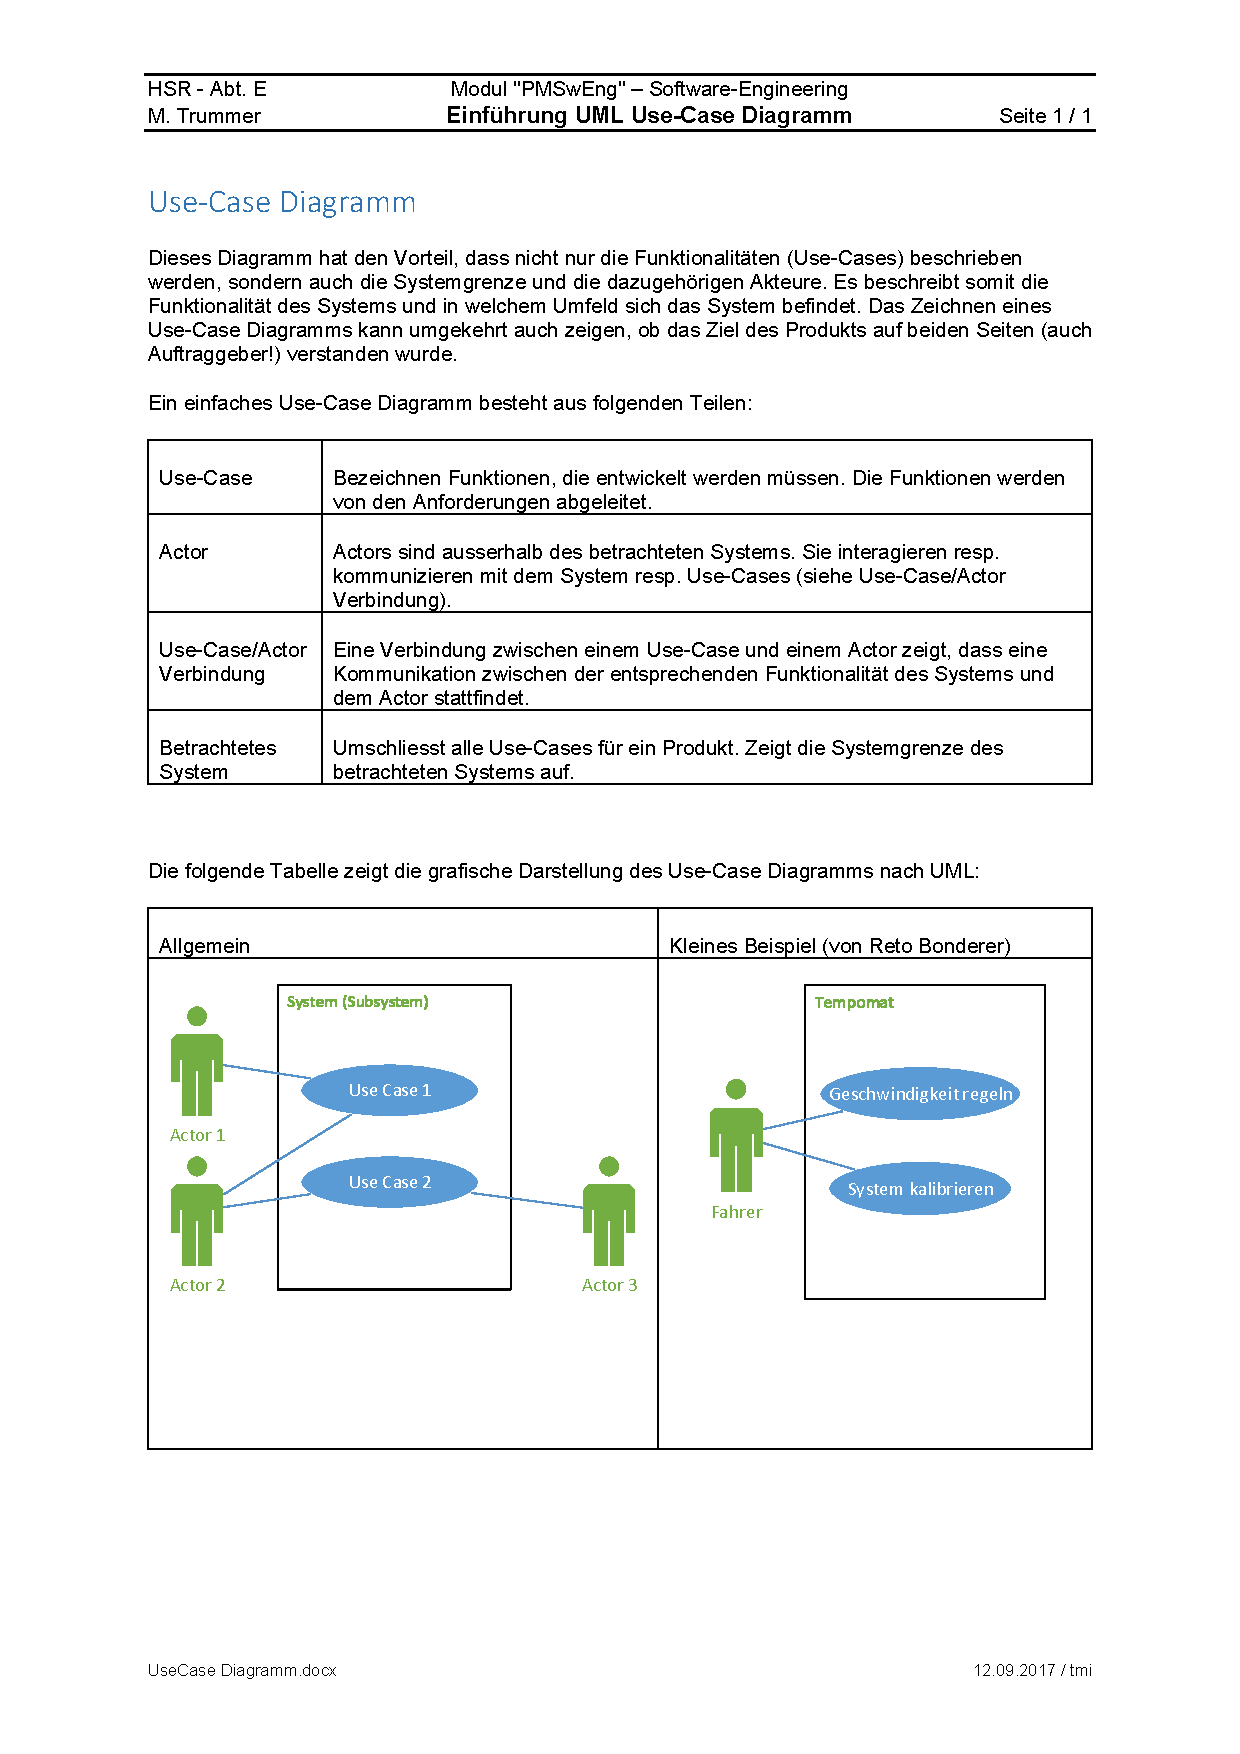
\includepdf[pages=-]{./Uebungen/UseCaseDiagramm.pdf}

\chapter{Vorgehensmodelle}

\section{Vorgehensmodelle in der Softwareentwicklung}

Vorgehensmodelle beantworten die wesentlichen Fragen der 
Organisation. Sie beschreibt das systematische, ingenieurmässig und quantifizierbare Vorgehen, um Aufgaben einer 
bestimmten Art wiederholbar zu lösen. Vorgehensmodelle werden hauptsächlich während Projektdurchführungsphase verwendet. Sie bilden eine Grundlage für die weitere Planung, die Projektüberwachung und die Projektsteuerung.

Sie bilden ein Instrument zur Integration von Methoden wie RE (Requirements Engineering) und Testen. Sie können anhand der W-Fragen strukturiert werden: Wer (--> Rollenmodell) erarbeitet Womit (--> Werkzeug \& Standards) Was (--> Artefakt-/Produktmodell) bis Wann (--> Ablaufmodell: Phase) und Wie (--> Aktivitätsmodell) geht er dabei vor? 

\section{Grundsätzliche Vorgehensmodelle}

Für Softwareprojekte stehen eine Reihe grundsätzlicher Vorgehensmodelle zur Verfügung. Die Modelle sollten auf das Projekt zugeschnitten werden (tailoring). Die Wahl für ein Modell erfolgt aufgrund des Projektcharakters.  \\
- Phasenmodell \\
- Spiralmodell \\
- Prototyping \\
- Agile Methoden \\

\subsection{Phasenmodell}
Das Phasenmodell ist ein klassischer Ansatz für die Organisation der Software- und Hardware-Entwicklung. Jede Phase erzeugt ein Ergebnis / Meilenstein, auf dem die nächste Phase aufbaut.

\subsection{Wasserfall-Modell}

\textbf{Philosophie:}  Aufteilung anhand Schwerpunkten der Entwicklungstätigkeiten 

\textbf{Phasen:} Analyse und Anforderung, Architekturentwurf, Implementation, Verifikation und Integration sowie Betrieb und Wartung

\textbf{Vorteile:} \\
- Einfache, klare Struktur \\
- Weitgehende Übereinstimmung des Artefakt- und Prozessmodells --> Vereinfacht scheinbar Planung, Organisation und Steuerung 

\textbf{Nachteile:} \\
- Planungs- und Entwicklungsfehler werden spät bemerkt  \\
- Risiken werden (zu) spät erkannt \\
- Umplanungen stehen im Gegensatz zur Philosophie und sind kostspielig \\
- Eine Rückkopplung aus der Implementationsphase findet sehr spät statt
- Enorme Erfahrung ist/wäre notwendig
\begin{figure}[ht]
	\centering
\adjustbox{width=12cm}{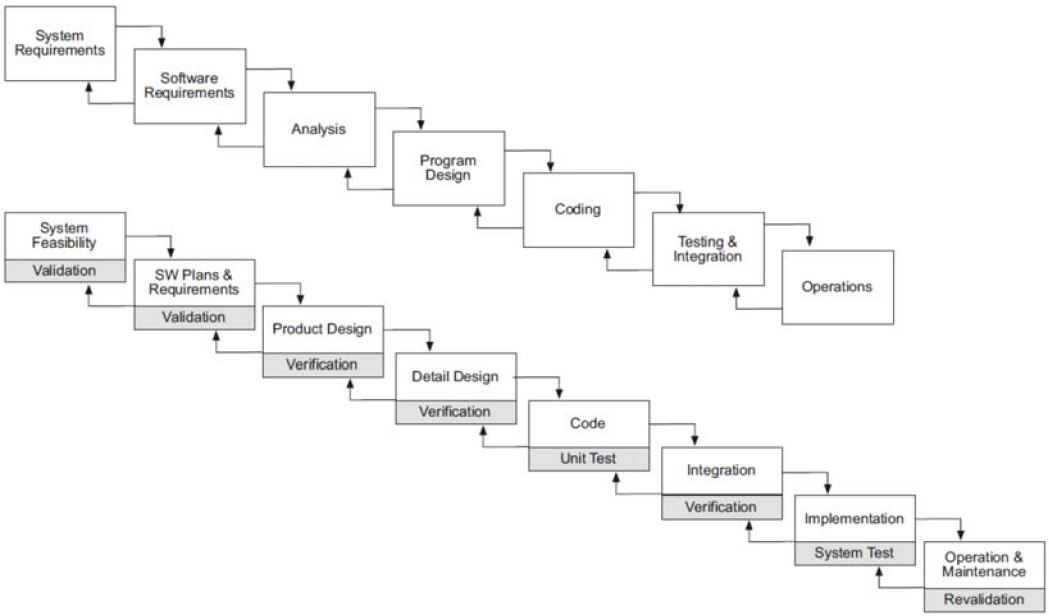
\includegraphics{Figures/wasserfall}}
\caption[]{Wasserfall - klassisch \& iterativ}
\end{figure}	
Iterativer Wasserfall: Kaskade; Erweiterung des Wasserfalls um Korrekturschleifen; In der Realität durchführbar (nicht wie der reine Wasserfall). Man kann immer nur eine Phase zurück

\subsection{V-Modell}
Grundidee: korrespondierende Tests \\
Erweiterung des Wasserfallmodells --> Ermahnt zum Testen
\begin{figure}[ht]
	\centering
	\adjustbox{width=8cm}{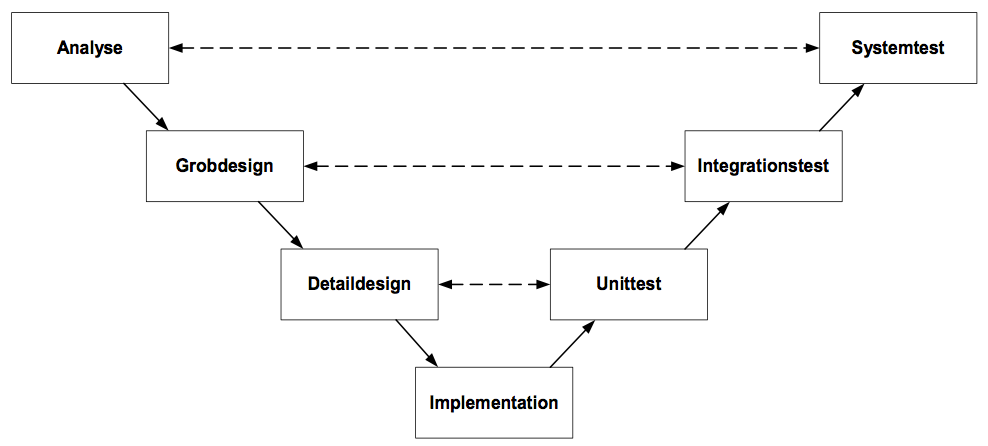
\includegraphics{Figures/v_modell}}
	\caption[]{V-Modell}
\end{figure}

\textbf{Vorteile:} \\
- Starke Einbindung der Test zu jeder Phase \\
- Klare, einfache Struktur \\
- Enorme Erfahrung aufgrund vorhandener Rückkopplung

\textbf{Nachteile:} \\
- kann zu inhaltlichen Problemen führen

\subsection{Spiralmodell}

Wiederholtes Durchlaufen der klassischen 
Entwicklungsphasen (Analyse, Evaluierung, Realisierung und Planung). Kontinuierliche Bereitstellung von 
Prototypen. Jede Iteration bringt den Prototypen näher 
an das endgültige Produkt. 

\textbf{Philosophie}
Erstellung von kontinuierlichen Prototypen und kontinuierliche Prüfung des System. Dies erlaubt kontinuierliche Lernkurven. Zudem werden die Ergebnisse der Zyklen wie Anforderungen oder Architekturen bei jeder Iteration verfeinert. Das weitere Vorgehen wird im 3. Schritt neu gewählt. Es ist kein Vorgehensmodell an sich, denn es sollte durch andere Vorgehensmodelle ausgestaltet werden. Im 4. Schritt kann allfällig eine Aufspaltung in Teilprojekte geschehen. 

\textbf{Inkrementelles Vorgehen} \\
Die Funktionalität wird schrittweise 
entwickelt bis das angestrebte System 
komplett ausgebaut ist. Iteratives Vorgehen ist zwingend nötig. 

\begin{figure}[ht]
	\centering
	\adjustbox{width=7cm}{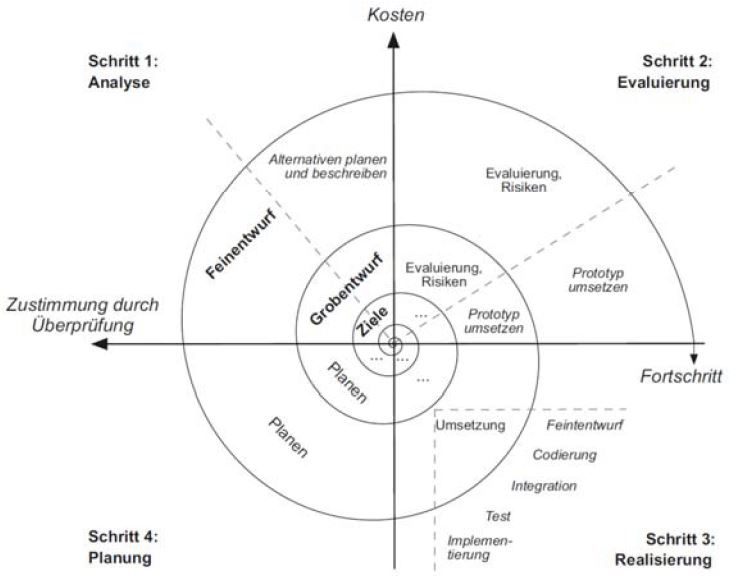
\includegraphics{Figures/spiralmodell}}
	\caption[]{Spiralmodell}
\end{figure}

\textbf{Vorteil:}
- Benötigt weniger Erfahrung als Wasserfallmodell, aufgrund der zugelassenen Lernkurven \\
- Risiken können frühzeitig erkannt werden

\subsection{Prototyping}
\begin{multicols}{2}
Prototyping beschreibt die frühe Realisierung ausgewählter oder kritischer Funktionen. Dabei geht es darum die Realisierung unter realitätsnahen Bedingungen zu zeigen. Es wird zur Prüfung der Machbarkeit, bei fehlender Erfahrung oder bei unklar definierten Anforderungen durchgeführt. \\
Anwendungen für Prototyping: bei User Interfaces, Smartphone Apps und Datenbanken
\columnbreak
Es wird zwischen einem horizontalem (Fokus auf eine Architekturebene) und vertikalen Prototyp (Fokus auf ein Funktionalität über alle Architekturebenen) unterschieden.
	\adjustbox{width=7.5cm}{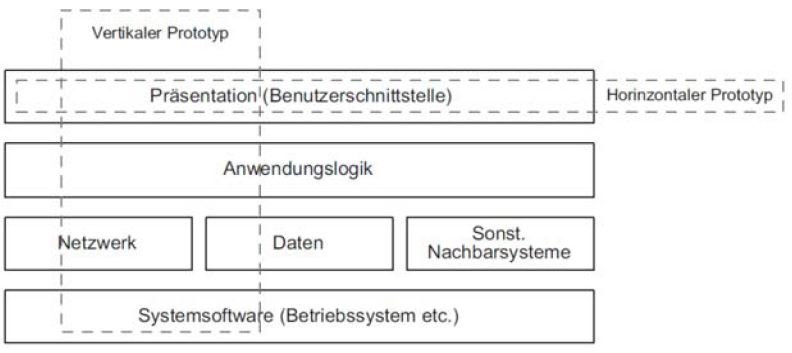
\includegraphics{Figures/formenvonprototyping}}

\end{multicols}

\subsection{Agile Methoden}
-  Gegensatz zu "schwergewichtigen" 
	Vorgehensweisen mit hohem Regelungs- und Organisationaufwand --> hohe Flexibilität, leichtgewichtiger Ansatz \\
- Agile = flink, beweglich / "Codezentriertes Vorgehen" \\

\textbf{Agiles Manifest (2001)}
- Individuen und Interaktionen mehr als 
Prozesse und Werkzeuge \\
- Funktionierende Software mehr als 
umfassende Dokumentation \\
- Zusammenarbeit mit dem Kunden mehr als 
Vertragsverhandlung \\
- Reagieren auf Veränderung mehr als das 
Befolgen eines Plans

Prominente Agile Methoden umfassen Refactoring, Pair Programming, Test-driven Development, Continuous Integration, Planning Game / Poker

\textbf{Vorteil:} \\
- Vorgehen kann für einen Hardware unabhängigen Teil der Software sinnvoll sein --> Stichwort "Hybrides Modell" \\
- Wertvolle Methoden: Refactoring / Test-Driven Development --> v.a. für erfahrene Programmierer

\textbf{Nachteil:} \\
Schwierig bei Hardwareentwicklung, da Anforderungen nicht zwingend von Anfang definiert

\section{Konkrete Vorgehensmodelle}
Die hier vorgestellten Modelle basieren auf den bereits gezeigten grundlegenden Philosophien. Die dabei grob beschriebenen Vorgehensmodelle eignen sich nur bedingt für die unmittelbare 
Anwendung in Projekten.


\subsection{Scrum}

Bei Scrum organisiert sich das Team weitgehend selbst. Die Grundannahme ist, dass Projekte komplex sind und somit nicht von Anfang an detailliert planbar sind. Am Anfang wird ein grober Projektrahmen definiert, indem sich das Team selbstorganisierend bewegt.

\begin{figure}[ht]
	\centering
	\adjustbox{width=10cm}{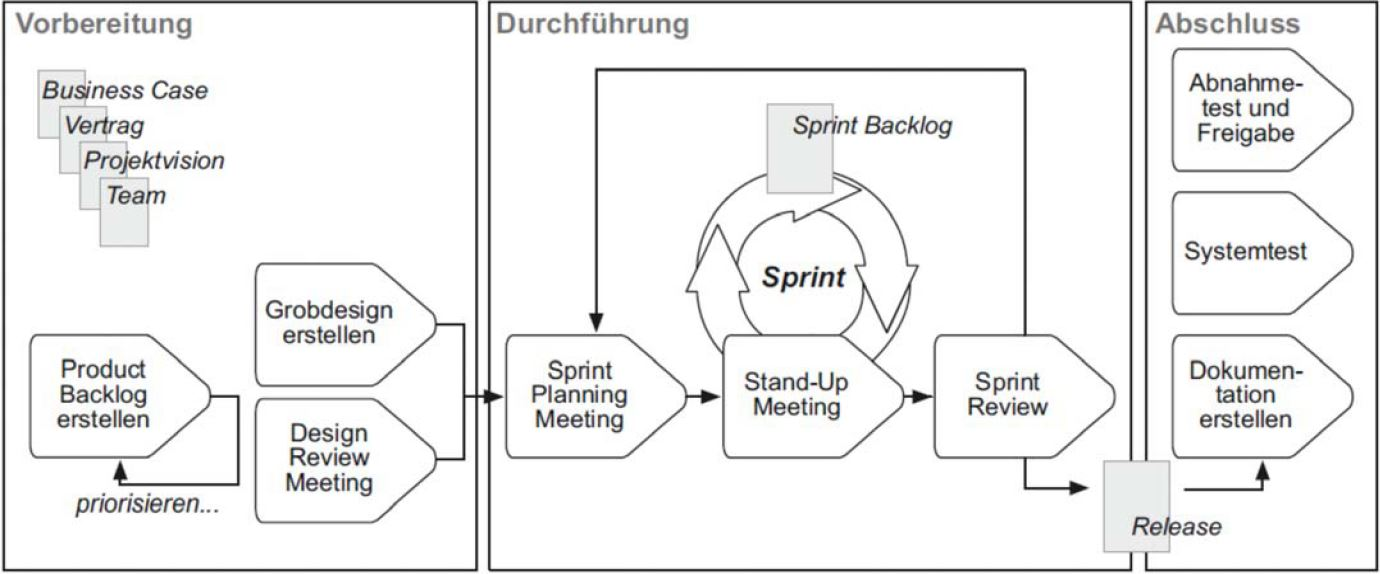
\includegraphics{Figures/scrum}}
	\caption[]{Scrum Prozess}
\end{figure} 
Basis: Sprints von 15-30 Tagen

\subsection{Rational Unified Process (RUP)}
RUP wurde von IBM Rational erfunden und wird kommerziell vertrieben. Es handelt sich um ein objektorientiertes, aktivitätsgetriebenes Vorgehensmodell, welches stark auf UML ausgerichtet ist. 
Grundprinzipien: \\
- Anwendungsfallgetrieben \\
-Die Architektur steht im Zentrum der Planung \\
- Das Vorgehen zur Entwicklung ist 
inkrementell/iterativ \\

\begin{figure}[ht]
	\centering
	\adjustbox{width=9cm}{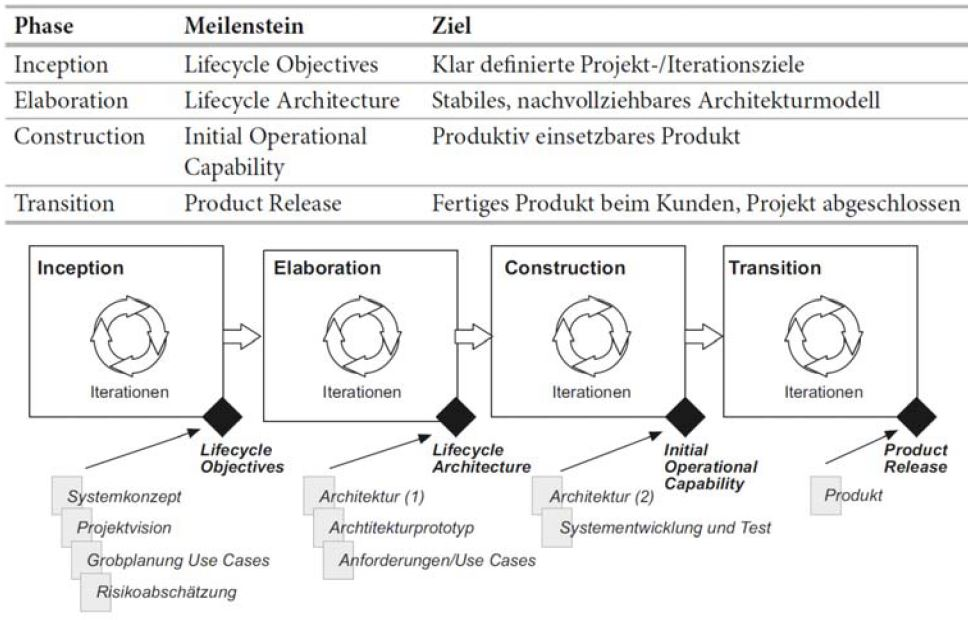
\includegraphics{Figures/RUP}}
\end{figure} 

\subsection{Diskussion der Vorgehensmodelle}
\begin{figure}[ht]
	\centering
	\adjustbox{width=15cm}{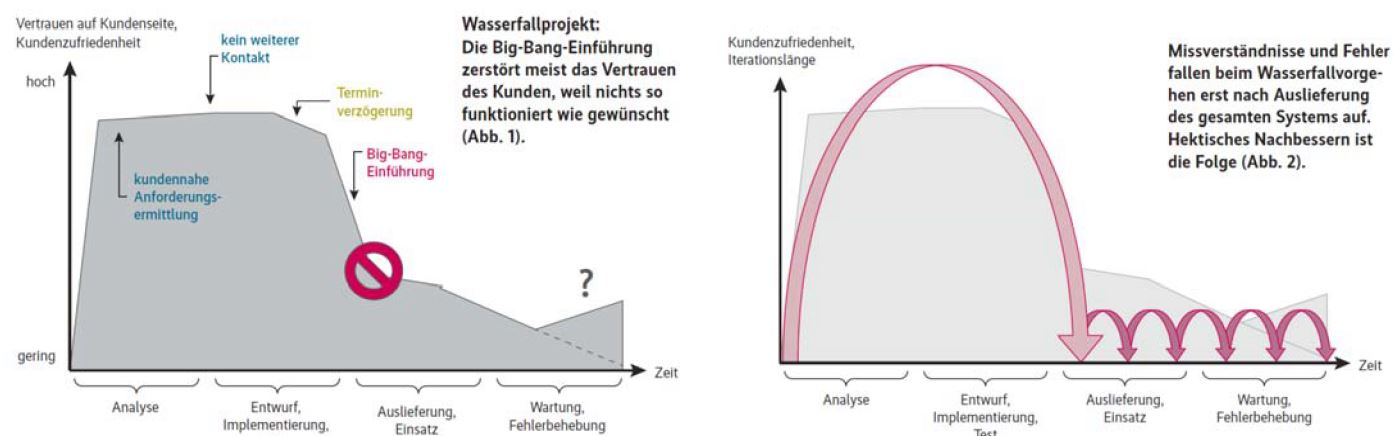
\includegraphics{Figures/diskussionvorgehensmodell}}
	\caption[]{Diskussion der Vorgehensmodelle}
\end{figure} 

\subsubsection{Brook'sche Regel}
\textit{Adding manpower to a late project makes it later} \\
Problem: Kommunikationsaufwand wird massiv erhöht.



\chapter{Aufwandsschätzung}

\section{Grundlagen}

Die Aufwandsschätzung ist ein kritischer, schwieriger und wichtiger Punkt in der Projektvorbereitung, -vereinbarung und -planung. Sie wird üblicherweise von sämtlichen Vertragsparteien unabhängig durchgeführt. Die Aufwandsschätzung bildet eine Grundlage für die Wirtschaftlichkeit, die Planung von Zeit und Projektmitteln und die Festlegung des erforderlichen Budgets. Der Projekterfolg hängt massgeblich von der Zuverlässigkeit der jeweiligen Schätzungen ab. 
Das Ziel von Schätzungen ist eine realistische Angabe über den erwartenden Aufwand und das erforderliche Budget zu machen.

Pessimistische Schätzungen sind oftmals wirtschaftlich uninteressant, da das Angebot nicht konkurrenzfähig ist. Sie beinhalten die Befürchtungen, dass Mittel und Freiräume dennoch ausgeschöpft werden (?).

Optimistische Schätzungen beinhalten ein grosses Risiko, da das Projekt meist nicht plangemäss durchgeführt werden kann. Sie können zu wirtschaftlichen Verlusten führen.

Aufwand- und Kostenabschätzung sollten sich am Umfang und der Besonderheiten des zu entwickelnden Ergebnisses orientieren. Dies kann die Software selbst, Dokumentation sowie Schulungsunterlagen sowie Dienstleistungen für Schulungen und Unterstützung bei der Einführung sein.

\textbf{Prinzipien bei Schätzungen}
\begin{itemize}
	\item Bildung von Schätzpaketen
	\item Aufwandseinheiten
	\item Einbindung der Mitarbeiter
	\item Dokumentation
	\item Erfahrungswerte und Aufschläge
	\item Kontinuierliche Kontrolle
\end{itemize}


\subsection{Schätzungsansätze}

\begin{minipage}{8cm}
	Aktivitätsorientierte Schätzung
\end{minipage}
\begin{minipage}{7cm}
	Artefaktbasierte Schätzung
\end{minipage}

\begin{figure}[ht]
	\centering
	\adjustbox{width=\textwidth}{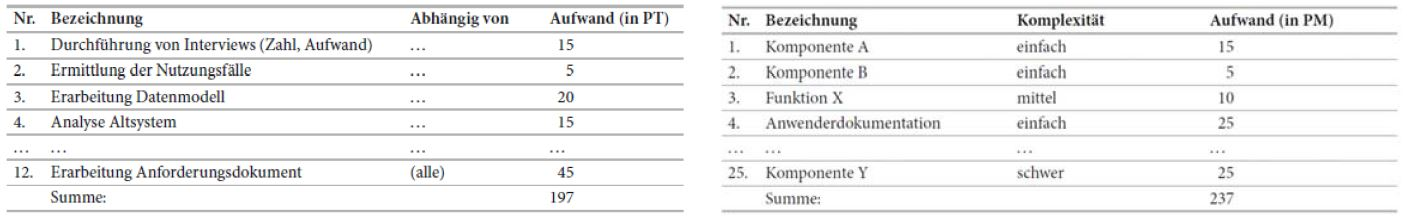
\includegraphics{Figures/schaetzungsansaetze}}
\end{figure}

\subsection{Streuung der Schätzung}

\begin{minipage}{8cm}
	Einflussfaktoren
\end{minipage}
\begin{minipage}{7cm}
	Leistungen in Abhängigkeit des Einsatzes
\end{minipage}

\begin{figure}[ht]
	\centering
	\adjustbox{width=\textwidth}{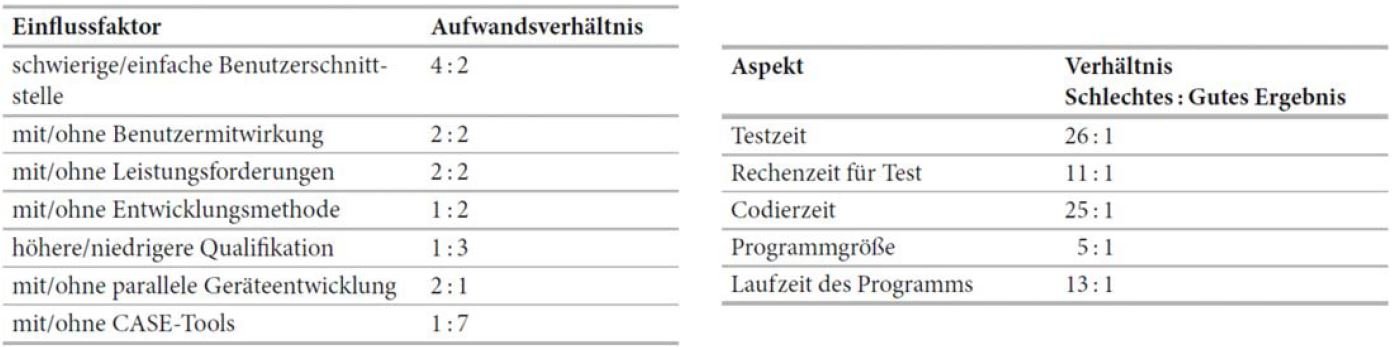
\includegraphics{Figures/streuung}}
\end{figure}

\section{Expertenschätzungen}
Die Expertenschätzungen finden an einer Schätzklausur statt. Dabei führen alle Beteiligten die Schätzung gemeinsam durch. Das Ziel ist dabei realistische Schätzergebnisse mit hoher Genauigkeit unter Berücksichtigung aller relevanten Faktoren zu erzielen. Ausserdem verspricht man sich dabei eine hohe Akzeptanz bei den späteren Projektmitarbeitern. 

\begin{minipage}{8cm}
	\textbf{Delphi Methode}
\end{minipage}
\begin{minipage}{7cm}
	\textbf{Planning Poker}
\end{minipage}

\begin{figure}[hb]
	\centering
	\adjustbox{width=0.49\textwidth}{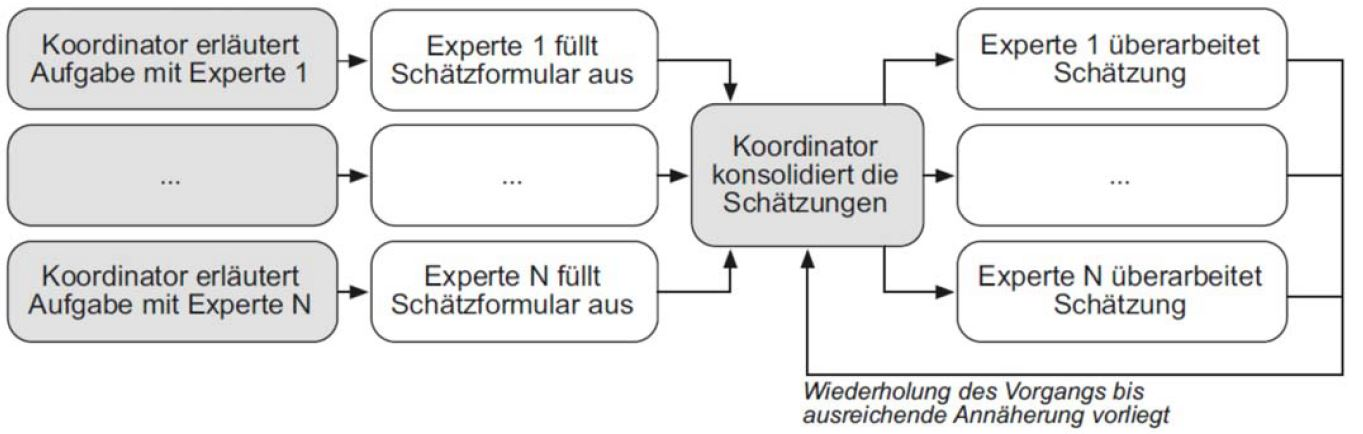
\includegraphics{Figures/delphimethode}}
	\adjustbox{width=0.49\textwidth}{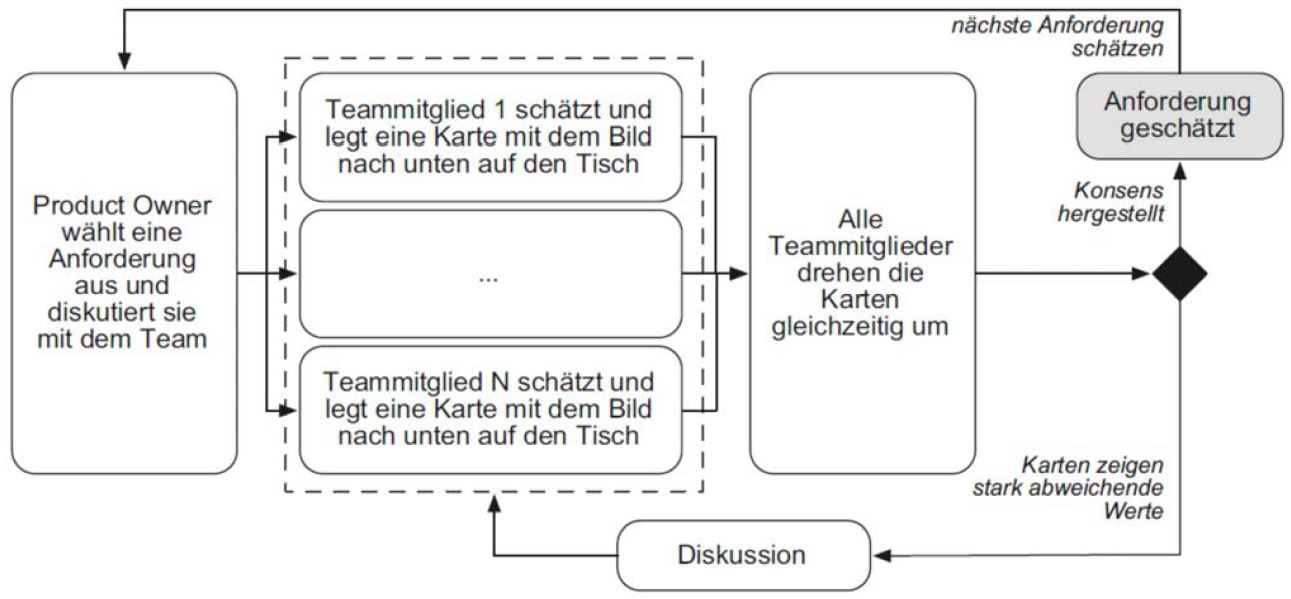
\includegraphics{Figures/planningpoker}}
\end{figure}

\subsection{Drei-Zeiten-Methode (nach PERT) zur Gewichtung von Schätzungen}

Aufwandsmittelwert für Schätzobjekt i: $A_i = \frac{bc_i + 4 lc_i + wc}{6}$ \\
Standardabweichung für Schätzobjekt i: $S_i = \frac{wc_i - bc_i}{6}$ \\
bc: optimistische Schätzung (best case) \\
wc: pessimistische Schätzung (worst case) \\
lc: wahrscheinliche Schätzung (most likely case) 

\section{Algorithmische Schätzverfahren}

\begin{itemize}
	\item Aron-Modell: (Selbststudium) Broy Kap. 6.3.3.1
	\item COCOMO: (Selbststudium) Broy Kap. 6.3.3.2, Hummel Kap. COCOMO S. 70 ff
	\item COCOMO II: (Selbststudium) Broy Kap. 6.3.3.2, Hummel Kap. COCOMO S. 70 ff
	\item Lines of Code (LOC)
	\item Function Points
	\item Speziell für Embedded: 3D Function Points oder COSMIC Full Function Points
\end{itemize}

\subsection{Function Points}
Function Points dienen der Schätzung des Umfangs der geforderten Funktionalität. Die zu schätzende Software wird als Black Box betrachtet, weshalb die Schätzung über die Schnittstellen, mit denen das System mit seiner Umwelt interagiert, erfolgt. 

\textbf{Datenelemente}
\begin{itemize}
	\item (ILF): Internal Logical Files
	\item (ELF): External Interface Files
	\item Data Element Types (DET): für den Systembenutzer sichtbare Datenfelder (z.B. Attribute von Klassen)
	\item Record Element Types (RET): Mehrere logisch zusammenhängende DETs ergeben einen RET
\end{itemize}
DETs und RETs sind verfeinernde Elemente für ILFs und EIFs.

\newpage

\textbf{Transaktionselemente}:
\begin{itemize}
	\item External Input (EI): von dem Benutzer oder einer umgebenden Applikation an die zu schätzende Applikation
	\item External Output (EO): von der zu schätzenden Applikation an den Benutzer oder eine umgebende Applikation
	\item External Query (EQ): Abfrage zwischen Benutzer oder umgebende Applikation und der zu schätzenden Applikation
\end{itemize}

\begin{figure}[hb]
	\centering
	\adjustbox{width=12cm}{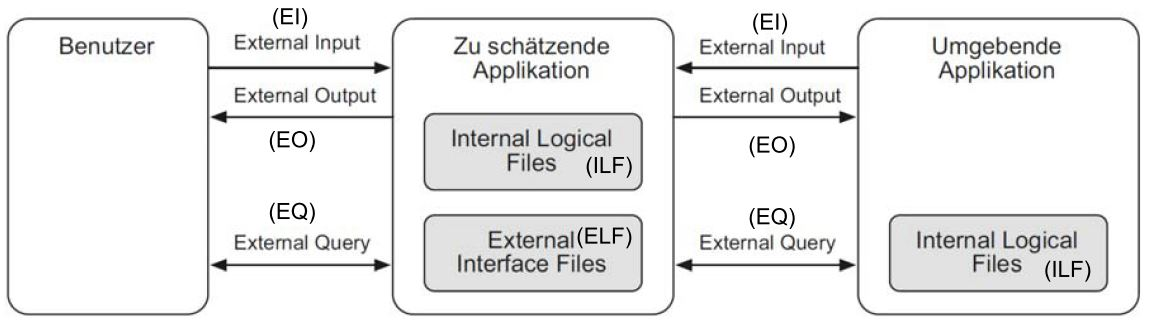
\includegraphics{Figures/transaktionselemente}}
	\caption[]{Daten- und Transaktionselemente}
\end{figure}

\subsubsection{Vorgehen}
Voraussetzung: Die Anforderungen müssen bekannt sein (unabhängig vom Detaillierungsgrad)
\begin{enumerate}
	\item Use-Case Diagramm erstellen: Festlegen der Systemgrenze
	\item Identifikation der Datenelemente (ILF, EIF)
	\item Identfikation der Transaktionselemente (EI, EO, EQ) 
	\item Berechnung der Unadjusted Function Points
\end{enumerate}


\subsubsection{Beispiel zu den Function Pointers}
\begin{figure}
	\centering
	\adjustbox{width=8cm}{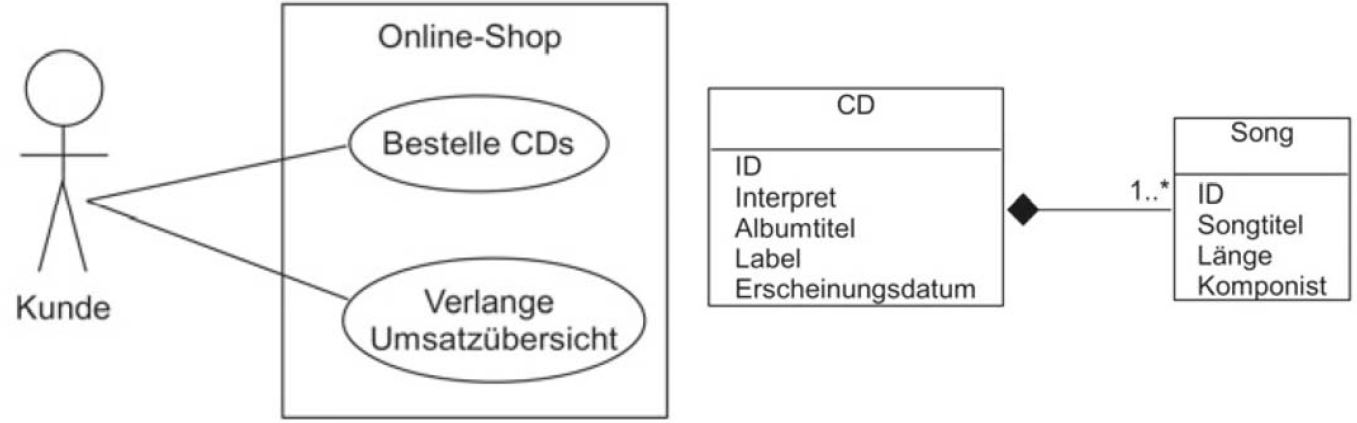
\includegraphics{Figures/fp1}}
\end{figure}
\newpage

\begin{multicols}{2}

\adjustbox{width=0.49\textwidth}{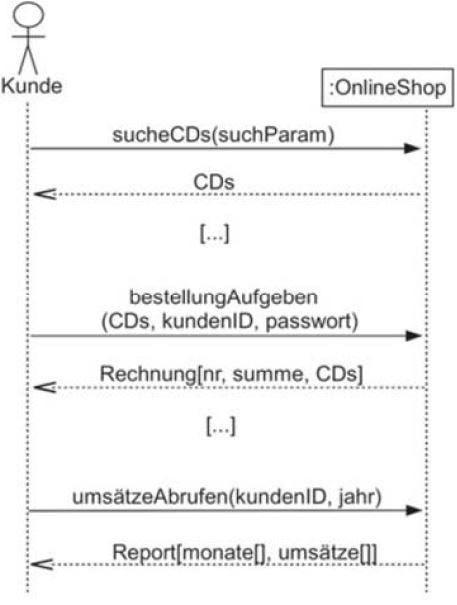
\includegraphics{Figures/fp2}}

\columnbreak
\textbf{Datenelemente} \\
Internal Logical File (ILF): \\
CD; 2 RETs (CD+Song) \\
- CD hat 5 DETs (Attribute von CD) \\
- Song hat 4 DETs (Attribute von Song) \\
DET total: 5+4 DETs (CD + Song)\\
Function Point Rating (FTRs): gering \\
\textbf{Transaktionselemente} \\
- sucheCDs (EQ): 1 FTR (CD), 7 DETs (alle CD Attribute + PushBtn click + Parameter) => geringe Komplexität = 3 FP \\
- bestellungAufgeben (EI): 4 FTR (Kunde, CD, Bestellung, Rechnung), 6 DETs (CD-ID, KundenID, Passwort, PushBtn click, RechnungsNr, Rechnungssumme) => hohe Komplexität: 6 FP \\
- umsätzeAbrufen (EO): 2 FTR(Kunde, Rechnung), 5 DETs(KundenID, Jahr, Monate, Umsätze, PushBtn click) => geringe K.: 4 FP	
\end{multicols}

\subsection{Bewertungslisten}

\begin{minipage}{8cm}
	\textbf{Funktionpoints pro Komplexitätsstufe}
\end{minipage}
\begin{minipage}{7cm}
	\textbf{Komplexität pro Anzahl RETs \& DETs}
\end{minipage}

\begin{figure}[hb]
	\centering
	\adjustbox{width=7cm}{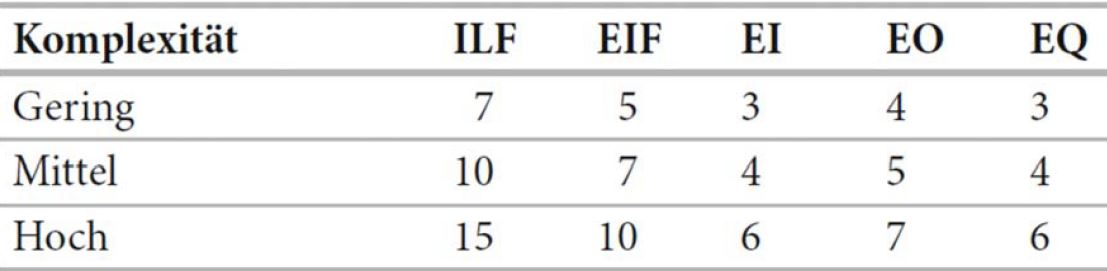
\includegraphics{Figures/Komplexitaet}}
	\adjustbox{width=7cm}{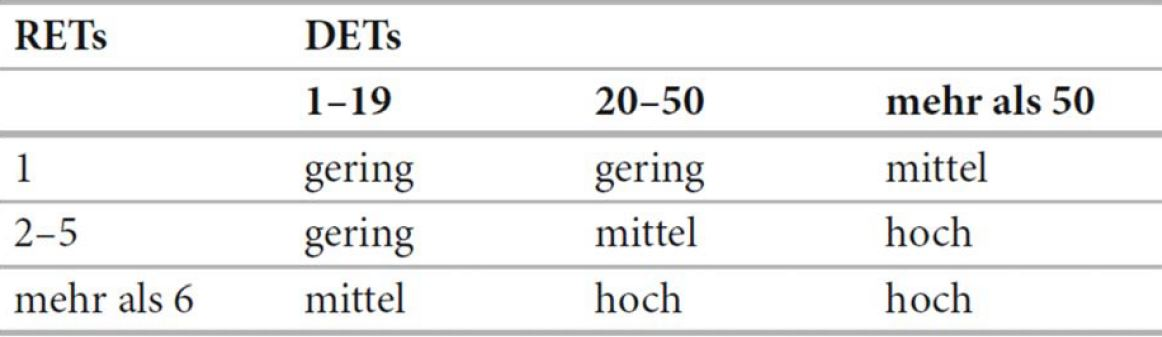
\includegraphics{Figures/RTSDET}}
\end{figure}

\begin{minipage}{8cm}
	\textbf{Function Points Ratings für EI}
\end{minipage}
\begin{minipage}{7cm}
	\textbf{Function Points Ratings für EO und EQ}
\end{minipage}

\begin{figure}[hb]
	\centering
	\adjustbox{width=7cm}{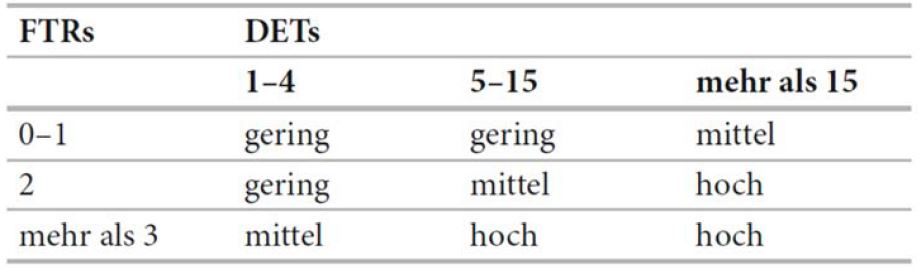
\includegraphics{Figures/FRRfuerEI}}
	\adjustbox{width=7cm}{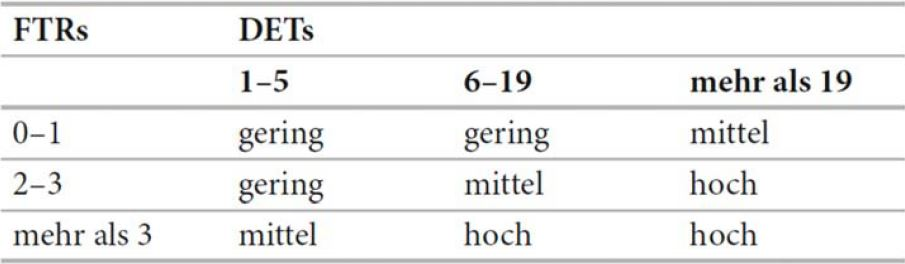
\includegraphics{Figures/FTRfuerEOEQ}}
\end{figure}


\section{Aron (Selbststudium), Broy Kap. 6.3.3.1}

\section{COCOMO (Selbststudium), Broy Kap. 6.3.3.2, Hummel Kap. COCOMO S. 70 ff}

\section{COCOMO II (Selbststudium), Broy Kap. 6.3.3.2, Hummel Kap. COCOMO S. 70 ff}
\chapter{Projektplanung}

Planung ersetzt den Zufall durch den Irrtum. Albert Einstein \\
Plans are nothing; planning is everything." - Dwight D. Eisenhower \\
"Plane – und du wirst irren. Plane nicht – und du wirst nicht wissen, wo du geirrt hast."
\section{Projekt- und Arbeitsplanung}

\subsection{Kernbestandteile der Projektplanung}
\begin{itemize}
	\item Projektstrukturplan - Aufteilung in Themenblöcke: \\ 
	- Phasenorientiert: Anforderungerhebung, Architektur \& Design, Implementation \\
	- Objektorientiert: Benutzerschnittstelle, Datenhaltung, Anwendungsfunktionalität, Kommunikation, Systemdienste \\
	- nach Verantwortung: QS, Fortschrittskontrolle, Anwendungs- und/oder Nutzungsfälle (Use Cases)
	\item Arbeitspakete \\
	beschreiben eine klar definierte Tätigkeit, definierte Dauer, zugeordnete Ressourcen sowie (logische oder zeitliche) Abhängigkeiten von anderen Arbeitspaketen 
	\item Zeit-/Terminplan (ggf. nur die nächsten Arbeitspakete "ausdetailieren")
	\item Meilensteinplan \\
	- Feststellen der Zielerreichung \\
	- Kann erfüllt oder nicht erfüllt sein \\
	- Blockierende Meilensteine (z.B. Projekt nicht genehmigt - Projekt steht still)\\
	-  Meilensteine sollten nicht zu nahe zusammenliegen)
	\item Schätzungen (siehe VL 7 Aufwandsschätzung)
\end{itemize}

Der Inhalt von Arbeitspaketen umfasst einen eindeutigen Identifikator, einen Namen zur Bezeichnung, eine Beschreibung des Arbeitspakets, Verantwortliche und mitwirkende Rollen/Personen, die geschätzte Dauer des Arbeitspakets, Ergebnisdefinition (geforderte Artefakte), Qualitätsanforderungen, Abnahmekriterien, technische Abhängigkeiten sowie zu erfassende Kennzahlen


\begin{figure}[ht]
	\centering
	\adjustbox{width=11cm}{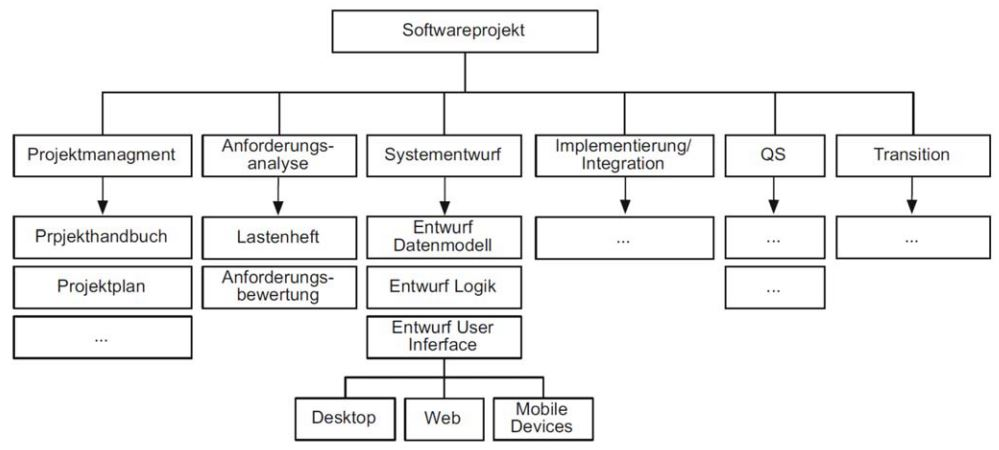
\includegraphics{Figures/Projektstrukturplan}}
	\caption[]{Projektstrukturplan}
\end{figure}

\begin{figure}[ht]
	\centering
	\adjustbox{width=11cm}{\includegraphics{Figures/Meilensteinplan}}
	\caption[]{Meilensteinplan}
\end{figure}

\subsection{Netzplantechnik}
 Grafische Darstellung der Zeitpunkte für die Durchführung von Tätigkeiten \\
 Logische Beziehungen und zeitliche Anordnung zwischen den Arbeitspaketen wird dargestellt. \\
Wie lange wird das Projekt (mindestens) dauern?
Welche kritischen Arbeitspakete können das gesamte Projekt verzögern?

\textbf{Methoden}
\begin{multicols}{2}
\begin{itemize}
	\item Critical Path Method
	\item Program Evaluation Review Technique (PERT)
	\item Meta Potential Method (MPM)  
\end{itemize}
\columnbreak

	\adjustbox{width=4cm}{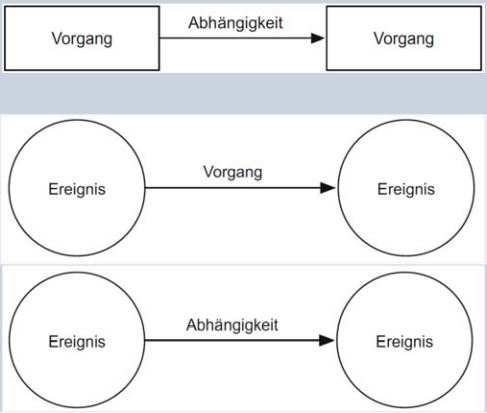
\includegraphics{Figures/npmethoden}}

\end{multicols}

\textbf{Modellierung} \\
Kritischer Pfad berechnen:
Wie in Digitaltechnik - Zeiten berechnen für ein Signal im Netzwerk.
Verkettung von derjenigen Vorgänge, bei 
deren zeitlicher Änderung sich der 
Endtermin des Netzplanes verschiebt. Aktivität a liegt auf einem kritischen Pfad bei p(a) = 0. Falls es keinen Projekt-Endtermin gibt hat man mindestens einen kritischen Pfad.

Vorwärtsrechnung: \\
Frühster Endtermin fet(a): Frühster Anfangstermin fat(a) + Vorgangsdauer d(a)

Rückwärtsrechnung: \\
Spätester Anfangstermin sat(a) = spätester Endtermin set(a) - Vorgangsdauer d(a)

Puffer: \\
Zeitdauer in der man die Aktivität herum schieben kann, ohne, dass sich das Projekt verzögert.
\\ Puffer p(a) = spätester Endtermin set(a) - frühster Endtermin fet(a) \\
 = spätester Anfangstermin sat(a) - frühster Anfangstermin fat(a)

\subsection{Balkenplantechnik - Gantt-Diagramm}

\begin{minipage}{7.5cm}
	Normalfolge: End-Anfang-Beziehung \\
	B startet wenn A fertig ist
\end{minipage}
\begin{minipage}{7.4cm}
	Anfangsfolge: Anfang-Anfang-Beziehung \\
	A und B müssen zeitgleich starten
\end{minipage}

\adjustbox{width=7.5cm}{\includegraphics{Figures/normalfolge}}
\adjustbox{width=7.4cm}{\includegraphics{Figures/anfangsfolge}}


\begin{minipage}{7.5cm}
	Endfolge: End-End-Beziehung \\
	A und B müssen zeitgleich beendet werden
\end{minipage}
\begin{minipage}{7.4cm}
	Sprungfolge: Anfang-End-Beziehung \\
	B kann erst beendet werden, wenn A anfängt
\end{minipage}

\adjustbox{width=7.5cm}{\includegraphics{Figures/endfolge}}
\adjustbox{width=7.4cm}{\includegraphics{Figures/sprungfolge}}

\subsubsection{Projektplanung in der Praxis}
- Netzpläne: für Grobplanung und prozessorientierte Darstellung \\
- Arbeitspakete werden oft zu stark unterteilt, Arbeitspakete mit Dauer < 1 Woche sollten ggf. überdacht werden \\
- Keine Abhängigkeiten zwischen Arbeitspaketen, wo keine notwendig sind: \\
--> Zuerst Pflichtenheft erstellen, dann Design / Implementation (Abhängigkeit) \\
--> Implementation und Test können parallel gemacht werden (keine Abhängigkeit) \\
--> Lieber eine Abhängigkeit weniger machen

Es gibt verschiedene Philosophien zur Projektplanung. Darunter sind Meilenstein-orientierte Planung, Fast Tracking, Time Boxing, Critical Chain und Kanban.





\chapter{Requirements Engineering}
Requirements Engineering heisst es Anforderungen an ein neues Softwareprodukt ermitteln, spezifizieren, analysieren und validieren. Daraus soll eine fachliche Lösung abgeleitet werden. 

\section{Vom Problem zur Lösung}
\begin{minipage}{10cm}
	\adjustbox{width=10cm}{\includegraphics{Figures/Probleml}}
\end{minipage}
\begin{minipage}{7cm}
	Elemente davon sind: 
	\begin{itemize}
		\item Anforderungen: Pflichtenheft
		\item Fachliche Lösung: OOA-Modell
		\item Technische Lösung: OOD-Modell
	\end{itemize}
Das OOA- und OOD-Modell sind Thema im Modul OOAD. 
Je weitere im Prozess, desto stärker wird der Lösungsraum eingeschränkt, wobei der Detaillierungsgrad der Lösung zeitgleich steigt. 
\end{minipage}

\subsection{Hauptgründe für einen Projektabbruch} 
- Änderungen der Anforderungen - 33 \% \\
- Mangelnde Einbindung des höheren Managements - 33 \% (Top Mgmt Committment) \\
- Engpass im Budget - 28 \% \\
- Fehlende Projektmanagement-Fähigkeiten - 28\% \\
--> Siehe Bild zu den "Relativen Bugfixing Kosten"

\section{Anforderungen und Anforderungsarten}
Die Anforderungen legen fest, was man (Stakeholder / Auftraggeber) von einem Softwaresystem als Eigenschaft (Visionen, Ziele, Rahmenbedingungen) erwartet. Eigenschaften lassen sich in funktionale und nichtfunktionale Anforderungen unterteilen. 
Die Anforderungsspezifikationen werden bei der Projektausschreibung in Lasten- und 
Pflichtenheft unterteilt. \\
\begin{minipage}{10cm}
	\adjustbox{width=10cm}{\includegraphics{Figures/anforderungsspezifikation}}
\end{minipage}
\begin{minipage}{7cm}
	\textbf{Lastenheft} \\
	- Zusammenstellung der Anforderungen \\
	- WAS und WOFÜR aus Sicht des Auftraggebers \\
	\textbf{Pflichtenheft} \\
	- Beschreibung der Realisierung der Anforderungen vom Lastenheft \\
	\textbf{Vision} \\
	- Beschreibt eine realitätsnahe Vorstellung der gewünschten Zukunft \\
	- Sie beschreibt, was erreicht werden soll, sagt aber nicht wie \\
\end{minipage}

\textbf{Regeln zur Definition von Zielen:}\\
Ausgehend von einer Vision dienen Ziele dazu, die Vision zu verfeinern und zu operationalisieren.
\begin{enumerate}
	\item Kurz und Prägnant --> Füllwörter vermeiden
	\item Aktivformulierungen verwenden --> Akteur klar benennen
	\item Überprüfbare Ziele formulieren --> Spezifisch
	\item Ziele, die nicht überprüft werden können, nicht verfeinern
	\item Den Mehrwert eines Ziels hervorheben
	\item Das Ziel sollte begründet werden --> Die Zielbegründung führt zur Identifikation weiterer Ziele
	\item Keine Lösungsansätze geben, da sie den Lösungsraum zu früh einschränken würden
\end{enumerate}

\textbf{Rahmenbedingungen} \\
Eine Rahmenbedingung – auch Restriktion genannt – legt organisatorische und/oder technische Restriktionen für das Softwaresystem und/oder den Entwicklungsprozess fest. 
\begin{multicols}{2}
\textbf{Organisatorische Rahmenbedingungen}
\begin{itemize}
	\item Anwendungsbereiche
	\item Zielgruppen
	\item Betriebsbedingungen
	\item Technische Rahmenbedingungen
\end{itemize}
\columnbreak
\textbf{Technische Produktumgebungen}
\begin{itemize}
	\item Welche SW / HW Komponenten sind auf der Zielmaschine
	\item Anforderungen an die Entwicklungsumgebung
	\item SW / HW
\end{itemize}
\end{multicols}

\textbf{Kontext und Überblick} \\
\begin{minipage}{10cm}
Festlegung der Einbettung in materielle und immaterielle Umgebung wie Sensoren, Personen, Übertragungsmedien, APIs, Internet zur Ermittlung der Systemgrenze (Use Case Diagramm). 
\end{minipage}
\begin{minipage}{5cm}
	\adjustbox{width=5cm}{\includegraphics{Figures/kontext}}
\end{minipage}

\textbf{Funktionale \& Nichtfunktionale Anforderungen} \\
\begin{multicols}{2}

\textbf{Funktionale Anforderungen}
\begin{itemize}
	\item das System beschreibende Anforderungen
	\item Statik
	\item Dynamik
	\item Logik
\end{itemize}
\columnbreak
\textbf{Nichtfunktionale Anforderungen}
\begin{itemize}
	\item Qualitätsanforderungen
	\item Genauigkeit, Verfügbarkeit, Zuverlässigkeit
	\item Sicherheit vs. Benutzbarkeit
	\item Speichereffizienz vs. Laufzeiteffizienz
\end{itemize}
\end{multicols}
Nichtfunktionale Anforderungen betreffen mehrere oder alle funktionalen Anforderungen und können sich gegenseitig beeinflussen

\textbf{Natürlichsprachliche Anforderungen} \\
Die Verwendung ist einfach \\
+ flexibel \\
- Synonyme (z.B. City – Innenstadt) und Homonyme (z.B. Bank) führen zu einer lexikalischen Mehrdeutigkeit

Syntaktische Mehrdeutigkeit \\
Die letzten 10 Buchungen und die Stornierungen des Kunden werden im Fenster angezeigt"

Semantische Mehrdeutigkeit \\
"Jeder Sensor ist mit einem Service verbunden" \\

Referentielle Mehrdeutigkeit \\
Beim Login muss zuerst das Benutzerkennzeichen und dann das Passwort eingegeben werden. Ist dies nicht korrekt, schlägt die Anmeldung fehl." \\

Vage Begriffe \\
Der Sensor muss neben der Tür angebracht werden" \\

Sprachliche Anforderungsschablone können verwendet werden.

\section{Anforderungsschablonen}

\begin{figure}[ht]
	\centering
	\adjustbox{width=\textwidth}{\includegraphics{Figures/ieee-schablone}}
	\caption[]{IEEE Schablone}
\end{figure}
%
%1 Einleitung (Introduction)
%Gibt einen Überblick über die Anforderungsdefinition.
%\begin{itemize}
%	\item 1.1 Zielsetzung (Purpose)
%	\item 1.2 Produktziele (Scope)
%	\item 1.3 Definitionen, Akronyme und Abkürzungen (Definitions, Acronyms and
%\end{itemize}
%
%Abbreviations)
%\begin{itemize}
%\item 1.4 Referenzen (References)
%\item 1.5 Überblick (Overview)
%\item 2 Übersichtsbeschreibung (Overall Description)
%\end{itemize}
%
%Gibt einen Überblick über das Produkt und die allgemeinen Faktoren, die seine Konzeption beeinflussen.
%\begin{itemize}
%\item 2.1 Produkt-Umgebung (Product Perspective)
%\item 2.2 Produkt-Funktionen (Product Functions)
%\item 2.3 Benutzer-Eigenschaften (User Characteristics)
%\item 2.4 Restriktionen (Constraints)
%\item 2.5 Annahmen und Abhängigkeiten (Assumptions and Dependencies)
%\end{itemize}

\textbf{3 Spezifische Anforderungen (Specific Requirements)} \\
Beschreibung aller Details, die für die Erstellung des System-Entwurfs benötigt werden. Das am besten geeignete Gliederungsschema dieses Kapitels 
hängt von der Anwendung und der zu spezifizierenden Software ab. Die IEEE-Richtlinie enthält dazu acht Vorschläge.\\
\begin{itemize}
	\item Externe Schnittstellen-Anforderungen (External Interface Requirements)
	\item Funktionale Anforderungen (Functional Requirements)
	\item Leistungsanforderungen (Performance Requirements)
	\item Entwurfsrestriktionen (Design Constraints)
	\item Eigenschaften des Softwaresystems (Software Systems Attributes)
	\item Andere Anforderungen (Other Requirements)
\end{itemize}

\section{Anforderungen ermitteln und spezifizieren}
\begin{figure}[ht]
	\centering
	\adjustbox{width=9cm}{\includegraphics{Figures/ProzesszurAnforderungsdefinition}}
	\caption[]{Prozess zur Anforderungsdefinition}
\end{figure}

\begin{figure}[ht]
	\centering
	\adjustbox{width=\textwidth}{\includegraphics{Figures/Stakeholderportfolio}}
	\caption[]{Stakeholderanalyse \& -portfolio}
\end{figure}

\subsection{Projektumfeld ermitteln}

Es geht darum das Umfeld des Projekts, welche das Projekt wesentlich beeinflussen können zu ermitteln. Das sind meist Vorgaben, Gesetze, Standards, Normen sowie ökologische, ökonomische, gesellschaftliche und kulturelle Einflüsse. 

\subsection{Anforderungen ermitteln}

Die Anforderungen können über Stakeholderbefragungen ermittelt werden. \\
- Erwarten Sie keine präzise Anforderung \\
- Erwarten Sie viel mehr schwammige, unvollständige, widersprüchliche Anforderungen \\
- Überlassen sie die Federführung für die Ermittlung von Anforderungen nicht einem Stakeholder \\

\textbf{Befragungstechniken} \\
- Strukturiertes Interview anhand Anforderungsschablone \\
- Selbstaufschreibung \\
- Stakeholder schreiben Arbeitsabläufe und Wünsche auf \\
- Analyse des Altsystems, falls vorhanden \\
 Die Ergebnisse der Anforderungsermittlung können nun systematisch ausgewertet und schrittweise in die Anforderungsschablone eingetragen werden

\section{Anforderungen priorisieren}

\textbf{Klassifizierung und Priorisierungsmethoden der Anforderungen} \\
-  Nach Kriterium: Häufig wir Notwendigkeit als Kriterium verwendet \\
- Mögliche Unterteilung nach IEEE830, S.13 in essenziell (essential), Bedingt notwendig (conditional), Optional (optional) \\

\textbf{Einige Priorisierungsmethoden} \\
- Ad-hoc Anordnung \\
- Reihenfolge der Anforderungen von Stakeholder oder Gruppe \\
- Top-Ten-Methode \\
- n-Anforderungen werden anhand Kriterium in Rangfolge gebracht
\newpage
\subsection{Kano-Modell}
\begin{multicols}{2}
	\adjustbox{width=6.9cm}{\includegraphics{Figures/kanomodell}} \\
\columnbreak
\\
Kano-Klassifikation \\
- Basiseigenschaft: vom Kunden implizit erwartet \\
- Leistungseigenschaft: vom  Kunden explizit gefordert \\
- Begeisterungseigenschaft: vom Kunden nicht erwartet \\ 
\end{multicols}
Das Kano-Modell kann auch für Anforderungen 
verwendet werden. \\
\begin{figure}[ht]
	\centering
	\adjustbox{width=\textwidth}{\includegraphics{Figures/kanomodell2}}
	\caption[]{Prozess zur Anforderungsdefinition}
\end{figure}
\chapter{Versionskontrolle Einführung - Git}

\section{Git}
\begin{itemize}
	\item Git = (engl.) Blödmann
	\item freie Software zur verteilten Versionsverwaltung von Dateien
	\item entwickelt für Quellcode-Verwaltung des Linus-Kernels
	\item Vokale Systeme: "Local Version Control Systems" (LVCS) -  SVN - Subversion \\
	\item Verteilte Systeme: "Distributed Version Control Systems" \\
	Mehrere verteilte Repositories für die zu archivierenden Dateien. 
	Bsp. Git \\
\end{itemize}

Ziele von Git
\begin{itemize}
	\item Geschwindigkeit
	\item Einfaches Design
	\item Vollständig verteilt (distributed Repository)
	\item Gute Unterstützung von nicht-linearer Entwicklung 
	\item ..
\end{itemize}

\subsection{Sicherungsart im Vergleich}
Git
\begin{itemize}
	\item stream of snapshots
	\item Speichert Snapshot von aktuellen Filesystem
	\item Link falls Datei nicht geändert (Pointer)
	\item Erst dann werden Deltas verwendet
\end{itemize}

SVN
\begin{itemize}
	\item Speichert die Datei beim ersten Mal und danach nur noch alle Änderungen
	\item Wird ein File aufgerufen, dann muss es erst das File erstellen und alle Änderungen durchführen
\end{itemize}

Bilder einfügen!

\subsection{Status von Dateien}
\begin{itemize}
	\item [committed:] Daten sicher gespeichert im lokalen Repo
	\item [modified:] Datei ist geändert zu (letztem Stand) aber nicht committed
	\item [staged:] Modifizierte Files ist markiert mit aktueller Version um im nächsten Commit-Snapshot zu gehen
	\item
\end{itemize}

\subsection{Bereiche}
\begin{itemize}
	\item Working Directory:
	\item Staging Area/ Index: 
	\item .git directory (lokal):
\end{itemize}

\subsection{Git Workflow}
Erstellen eines Ordners
\textbf{-mkdir gitTest} \\
Erstellen eines Git Repositories (.git Ordner):
\textbf{git init} \\
Erstellung eines lokalen Repositories erfolgt. \\

Tracked vs. Untracked: Dateien die Git bekannt sind. Die unter Versionsverwaltung stehen. 
Add the file
Edit the file
Stage the file
Commit the file
Remove the file

Übersicht über die aktuelle Lage im Repository: \textbf{git status} \\
Funktionalität: \\
Registerzustand aller Files, Aktueller lokaler Branch, Abweichungen vom entfernten Branch.

Hinzufügen eines Files, welches bereits in den entsprechenden Ordner gespeichert wurde: \textbf{git add <file name>} \\
Überprüfung der Aktion: \textbf{git status} \\
File dem Repository hinzufügen: \textbf{git commit -m "Comment"} \\
Fragt den Namen und die Email nach: \textbf{git config - global user} \\
Differenz zwischen Staging Area und Working Directory feststellen: \textbf{git diff <file name>} \\
Wiederum das File "stagen": \textbf{git add <file name>} \\
File dem Working Directory hinzufügen: \textbf{git commit -m "Comment"}
File aus der Versionsverwaltung raus nehmen: \textbf{git rm <file name"} \\
Histories anzeigen: \textbf{git log}

GUI: 
\begin{itemize}
	\item git gui
	\item gitk: "native gui" von git \\
	(Alle Branches werden angezeigt mit --all)
\end{itemize}

Commit Baum Darstellung: Jeder Commit hat einen eigenen Hash-Wert und es gibt dazu jeweils einen Snapshot. Branches sind Zeiger, die auf bestimmte Commits zeigen. Der Masterbranch zeigt auf den aktuellen Commit. 

Frühere Versionen zurückholen
Aus dem lokalen Repo wird etwas wieder in die Staging Area zurückgeholt: \textbf{git reset <path>} \\
Datei(en) "unstagen", indem die Dateiversion vom letzten Commit verwendet wird.  \\
Working Directory mit alter Version überschreiben: \textbf{git checkout HEAD path}

\subsection{git clone <URL>}
git clone https://git.hsr.ch/git/reponame
Beinhaltet folgende Schritte:
\begin{enumerate}
	\item Erstellt neues Verzeichnis
	\item Wechselt in das neu erstellte Verzeichnis
	\item Führt git init aus um lokales Repo zu erstellen
	\item Führt git remote add origin URL aus
	\item Führt git fetch aus
	\item Führt git checkout –b branch
	origin/branch ( HEAD vom remote Repo)
\end{enumerate}
Von einem entfernten Repo wird ein lokales Repo erstellt.

\subsection{git remote add <kurzname> <URL>}
Verbindung zu einem entfernten Repo erstellen. Bsp.: git remote add origin https://git.hsr.ch/git/gitTest \\
per default wird origin als Kurznamen für ein 
remote Repo verwendet \\
Normalerweise verwendet man git clone und nicht git remote. \\

\subsection{git fetch <remotename>}
Aktualisiert lokales Repo vom Remote Repo. Bsp.: git fetch origin. \\
Die Commits, die wir schon hatten bleiben, werden jedoch als "Branch" zur aktualisierten Version des Remote Repo, welche wir ins lokale Repo geladen haben, angezeigt. Nun hat man jedoch 2 Zweige, welche wieder vereint werden sollen. 

\subsection{git pull}
Aktualisiert lokales Repo vom entfernten Repo und merged Änderungen zum lokalen Repo. 
Ist wie git fetch, jedoch werden die 2 Zweige ineinander verwoben "merge". //
git pull origin master entspricht git fetch origin \& git merge origin/branchname
Merge-Konflikte: Identische Codezeilen wurden geändert -> Manuelle Überprüfung der 2 Versionen und Entscheid für eine Version. 
Es ist wichtig, dass man modified files zuerst committed bevor man einen pull macht.

\subsection{git push}
Veröffentlich lokales Repo und der master-Branch wird aktualisiert. 
git push <remotename> <branchname>


\section{Tagging}

\subsection{git tag}
Tags sind da, um spezifische Punke in der History zu taggen.

\begin{itemize}
	\item Lightweight Tag \\
	git tag -a v2.3
	\item Annotated Tags (Kommentierter Tag) \\
	git tag -a v1.3 -m "myComment"
\end{itemize}

\section{Branching}

Ein Branch ist ein verschiebbarer Zeiger
Es gibt HEAD-Zeiger und Tags.
Der Master Branch wird per Default erstellt.

\subsection{git branch <branchname>}
Erstellen eines neuen Branch.  Jedoch wird nicht auf diesen Branch gewechselt (Head bleibt stehen), 
git checkout <branchname> Head-Zeiger wird auf neuen Branch verschoben. 
Nun erfolgt ein commit auf einem Branch. 

git checkout master
Der Head-Zeiger ist wieder auf dem master-branch.
git commit - nun wird wieder etwas auf dem Master-branch committed. 
Es resultiert eine Verzweigung.

\subsection{git merge}
Zusammenführen von zwei Branches. Es gibt Fast-Forward merge: git merge <brachname>. Der master-branch-Zeiger wird entlang der Kette verschoben. Es resultiert kein Merge-Problem.
Three-way Merge: Merging-Konflikte sind möglich.
Git entscheidet selbst ob ein FF-merge oder ein three-way merge erfolgen soll.  \\
Mergekonflikte: \\
Mit GUI: KDiff3 mittels \textbf{mergetool} \\
Eine von beiden Dateien komplett verwenden: \textbf{git checkout \lbrack--theirs/--ours\rbrack}

\subsection{git reset}
Datei(en) «unstagen», indem die Dateiversion 
vom letzten commit verwendet wird \\
git reset path \\
git reset <filename>
\adjustbox{width=7cm}{\includegraphics{Figures/reset}}

\subsection{git checkout}
Working Directory mit alter Version 
überschreiben: git checkout HEAD path \\

File(s) in  Staging Area wird von local Repo
überschrieben: git checkout <filename> \\

File(s) in Staging Area und Working Directory 
wird von local Repo überschrieben: git checkout HEAD README \\
Achtung: Kann Daten zerstören


\subsection{gitignore}

Hinzufügen von Files mit bestimmten Endungen zu gitignore: \\
echo *.aux >> .gitignore \\
Files verwerfen, die bereits in der Staged Area sind: \\
git rm --cached <filename>
\chapter{Code Dokumentation mit Doxygen}

\section{Dokumentation \& Code-Dokumentation}

\subsection{Zweck der Dokumentation}

\begin{itemize}
	\item  Wissenssicherung: \\ Wissen über ein System macht einen beträchtlichen Wert des Systems aus --> Menschen vergessen schnell
	\item Förderung der Kommunikation \& Genauigkeit 
	\item Sichtbarmachen des  Projektfortschrittes: \\ Fertigstellung und Freigabe von Dokumenten markiert nachprüfbar(!) den Projektfortschritt
\end{itemize}

Bei der Programm-Dokumentation werden bestehende Programmteile (v.a. Schnittstellenbeschreibungen (APIs)) verwendet. Der Entwickler / Programmierer dokumentiert, wenn das bestehende Programm verändert wird.

Die Dokumentation im Code hat den Vorteil, dass Dokumentationen bei Änderungen häufig nicht nachgeführt wurden, da Code und Dokumentation getrennt waren. Dies führte zu Inkonsistenzen sowie fehlerhaften und unvollständigen Dokumentationen.

Code-Dokumentationen integrieren Beschreibungen in den Source-Code mit Hilfe von speziellen
Kommentaren. Die Dokumentation wird erzeugt mit Hilfe von Dokumentationswerkzeugen, die den Sourcecode analysieren und die Beschreibung daraus extrahieren.

\subsection{Vorteile von Code-Dokumentation}
\begin{itemize}
	\item Erzeugung der Dokumentation kann leicht automatisiert werden. --> Dokumentation bleibt aktuell
	\item Gewisse Informationen, wie z.B. Funktionsköpfe, werden direkt aus dem Programmcode 
	entnommen.  
	\item Dadurch, dass Beschreibungen und Source-Code unmittelbar nebeneinander im Source-Code-
	Dokument vorkommen, ist die Wahrscheinlichkeit gross, dass Programmcode und Beschreibung 
	übereinstimmen. --> Dokumentation bleibt konsistent
	\item Vor allem geeignet zur API-Dokumentation von Klassen bei der Objektorientierten 
	Programmierung.
	\item Hinweis auf gewisse nicht dokumentierte Codestellen (z.B. Parameter) leichter. --> Dokumentation ist vollständig
\end{itemize}

\section{Doxygen}
- The KDE API Reference (Linux Desktop): http://api.kde.org/ \\
- D-Bus documentation (SW Message Bus System): http://freedesktop.org/software/dbus/doc/api/html/index.html \\
- The Xerces-C++ Documentation (XML-Parser): http://xerces.apache.org/xerces-c/apiDocs-3/classes.html \\

Weit verbreitetes Dokumentationswerkzeug:  \\
- Open Source, für Windows, Unix / Linux, Mac, … \\
- unterstützt: C, C++, Java, C\#, etc. \\

Erzeugt Dokumente in folgenden Formaten: \\
- HTML (für Browser) – am häufigsten \\
- LaTeX (dvi, pdf mit Links, PostScript …) \\
- Unix man pages \\
- RTF (MS-Word) \\
- XML (für maschinelle Weiterverarbeitung) \\
Erstellt primär API-Beschreibungen, aber (mit Zusätzen) auch Klassendiagramme und andere 
Diagramme. \\
Weitere Infos, Website:  http://www.stack.nl/~dimitri/doxygen/

\begin{figure}[ht]
	\centering
	\adjustbox{width=11cm}{\includegraphics{Figures/darchitektur}}
	\caption[]{Doxygen Architektur}
\end{figure}

Doxygen ist ein "Command-Line-Tool". \\
GUI-Frontend "doxywizard" sowie Plugins z.B. für Eclipse («Eclox») \\
Hauptbefehl (command-line): \$ doxygen \\
Doxygen benötigt eine Konfigurationsdatei: "Doxyfile" \\
Aktuelle Anzahl möglicher Konfigurationen: 267 \\ 
Aufruf-Beispiele: \\
\$ doxygen -g     // erzeugt Konfigurationsdatei "Doxyfile" \\
\$ doxygen Doxyfile // erzeugt Dokumentation, falls Konfig'datei Doxyfile heisst, reicht:\$ doxygen

\subsection{Wichtigste Einstellungen}
- Projektname: PROJECT\_NAME = "Voltage Divider" \\
- Input: INPUT = . ./src ./tests README.md \\
- Datei-Filter: FILE\_PATTERNS = *.cpp, *.h \\
- Output: OUTPUT\_DIRECTORY = doc \\
- README.md als mainpage: USE\_MDFILE\_AS\_MAINPAGE = README.md \\

\subsection{Wichtigste Befehle für Doxygen}
Allgemein \\
- Dateikopf \\
- file \\
- date \\
- author \\

Funktionsbeschreibung \\
- brief \\
- param \\
- pre \\
- post \\

Beispiel: \\
/// \textbackslash brief Calculates the optimal values for R1 and R2. The base formula \\
///        behind this calculation is \textbackslash f$u1=u2 {r2 \over r2+r1}\textbackslash f$. \\
/// \textbackslash pre \textbackslash p u1 > \textbackslash p u2 \\
/// \textbackslash pre \textbackslash p lowerRTh < \textbackslash p upperRTh \\
/// \textbackslash param u1 Value for U1 in V \\
/// \textbackslash param u2 Value for U2 in V \\
/// \textbackslash param lowerRTh set the lower bound for resistor value output \\
/// \textbackslash param upperRTh set the higher bound for resistor value output \\
/// \textbackslash param resDecade gives the resister e-decade on which the resistor are calculated  
virtual void calc(double u1, double u2, double lowerRTh, double upperRTh,
const EDecade\& resDecade); \\

\begin{figure}[ht]
	\centering
	\adjustbox{width=10cm}{\includegraphics{Figures/dhtmlausschnitt}}
	\caption[]{Ausschnitt aus dem HTML-Output}
\end{figure}


Die Doxygen Hauptseite wird als erstes in der HTML Dokumentation angezeigt. \\
Zweck: Sie soll einen Überblick über das gesamte Projekt vermitteln \\
Formatierungsanweisung:  @mainpage oder markdown file (z.B. README.md, empfohlen)

\subsection{Weitere Informationen zu Doxygen}
Ein Markdown-File (typischerweise README.md genannt) enthält eine Plain Text Formatierungssyntax. Das Ziel ist dabei es so leserlich wie möglich zu machen. Es soll als plain Text publiziert werden wie es ist, ohne visueller Überladung durch zusätzliche Syntax. \\
Beispiel: \# This is an H1 Header \# oder \#\# This is an H2 Header \#\# \\
Es kann kann mit folgendem Befehl verwendet werden: USE\_MDFILE\_AS\_MAINPAGE = README.md \\
INPUT = ./tests ./src README.md  \\
Die erste Zeile wird im Titelbalken dargestellt. Mit einem Punkt wird der Projektname verwendet. Der Nachteil bei dieser Lösung ist eine Warnung beim Übersetzten \\
Weitere Syntax: http://daringfireball.net/projects/markdown/syntax \\

\subsubsection{Code Documentation Style}

\begin{minipage}{8cm}
 Java / C 
\end{minipage}
\begin{minipage}{3cm}
	C
\end{minipage}
\begin{minipage}{3cm}
	C++
\end{minipage}
\begin{minipage}{3cm}
	C++
\end{minipage}

\adjustbox{width=8cm}{\includegraphics{Figures/textstylejava}}
\adjustbox{width=3cm}{\includegraphics{Figures/textstylec}}
\adjustbox{width=2cm}{\includegraphics{Figures/textstyle}}
\adjustbox{width=2cm}{\includegraphics{Figures/textstyle2}}

\textbackslash \textbackslash  sind hier wichtig. Sie schliessen einen normalen Kommentarblock und öffnen einen C-Style Kommentarblock. 

\subsubsection{Weitere Befehle für Doxygen}

Jeder Befehl beginnt mit @ oder \. \textbackslash wird häufig für C/C++ und @cmd oft für Java genutzt. 
LaTex Formeln sind kompatibel für Outputs in LaTeX und HTML. \\
Dabei muss USE\_MATHJAX eingeschaltet sein. \\
Beispiel: \textbackslash f\$formel\textbackslash f\$\\
Bilder sind kompatibel für Outputs in LaTeX, HTML, Docbook und Rtf. \\
Dabei muss IMAGE\_PATH auf den Pfad mit den Bildern zeigen. \\
Beispiel:  \textbackslash image format file "caption" \\
\textbackslash image html Kontextdiagramm.gif "Kontext-Diagramm" \\
\textbackslash image latex Kontextdiagramm.eps "Kontext-Diagramm" width=10cm \\

\chapter{Testing \& Unit Testing}
Definition:
Testen ist der Prozess, ein Programm mit der Absicht auszuführen, Fehler zu finden.(G. J. Myers, The Art of Software Testing, 1979)\\
"To test a program is to make it fail." – Bertrand Meyer, 2008 \\
Jeder durch Testen gefundene Fehler ist ein Erfolg. Nach sorgfältigem Testen eines Programms steigt die Wahrscheinlichkeit, dass das Programm sich auch in nicht getesteten Fällen wunschgemäss verhält. Durch das Testen kann die Korrektheit eines Programms aber nicht bewiesen werden.

Je mehr Fehler gefunden werden, umso 
höher ist die Wahrscheinlichkeit für weitere 
Fehler.
\begin{figure}[hb]
	\centering
		\adjustbox{width=0.5\textwidth}{\includegraphics{Figures/error}}
\end{figure}


\subsection{Testen versus Debugging}
Ziel von Testen: \\
Aufzeigen, beweisen, dass Fehler (Bugs) 
existieren --> Destruktives Testen \\
"Jeder gefundene Bug ist ein Gold-Nugget!"

Ziel von Debugging: \\
Die durch Testen gefundenen Bugs beseitigen

\subsection{Laufversuch versus systematischer Test}
Laufversuch
\begin{itemize}
	\item Entwickler testet Code während Implementation 
	fortlaufend
	\item Kann mittels Debugging festgestellt werden
	\item Fehler werden sofort korrigiert
\end{itemize}
	Ist wichtig um zu überprüfen, ob das Programm 
das tut was man will

Systematischer Test
\begin{itemize}
	\item Systematische Fehlersuche
	\item Test werden geplant
	\item SOLL wird mit IST verglichen
	\item Resultate  werden festgehalten
	\item Wenn möglich nicht durch Entwickler der 
	Software
\end{itemize}
Ist wichtig um die Richtigkeit einer Software 
jederzeit reproduzieren und nachvollziehen zu 
können

\subsection{Testarten}

\textbf{Abnahmetest} (Anforderungen; Kunde): Validierung, Besondere Test-Form, Soll nicht Fehler aufzeigen, sondern zeigen, dass das System nach Anforderungen
(gemäss Pflichtenheft) fehlerfrei funktioniert \\
\textbf{Systemtest (Architektur; Tester):} Test des gesamten Systems (z.B. inkl. Mechanik) \\ \textbf{Integrationstest (Entwurf; Entwickler/Tester):} Integration von Programmeinheiten \\
\textbf{Modultest (Detailentwurf/Implementation; Entwickler):} Unit-Test

Die Tests sollten entsprechend den verschiedenen Phasen gemacht werden (Phase und Aktor in Klammern geschrieben). 

\subsection{Verifikation und Validierung}
 Validierung  (Validation)
"Are we building the right product?"
Überprüft das Software-Produkt,
ob es die Anforderungen des Auftraggebers erfüllt.

Verifikation (Verification): 
"Are we building the product right?"
Überprüft die Artifacts während der Entwicklung,
ob sie ihre Vorgaben erfüllen
(Artifacts = künstliche, d.h. von Menschenhand geschaffene Dinge wie Dokumente etc.)

\subsection{Prinzipieller Ablauf eines Tests}
\begin{multicols}{2}
	\adjustbox{width=0.35\textwidth}{\includegraphics{Figures/testplan}}
\columnbreak

Vorzüge von einem Testablauf: 
\begin{itemize}
	\item  Reproduzierbar
	 \item Wissen, was getestet wurde
	\item Unabhängig von testender Person
	\item Wenn möglich automatisiert
	\item Testspezifikation fortlaufend erweitern
\end{itemize}
\end{multicols}
\subsection{Testspezifikation / Testprotokoll}
Redundanz vermeiden; Möglichst in Code integrieren oder/und 
automatisieren

Elemente: \\
Test-Spezifikation (Test-Code) \\
Test-Protokoll: Wird typischerweise von Test-Frameworks 
erstellt \\
Test-Dokumentation (z.B. mit Hilfe von Doxygen)

\subsection{Auswahl der Testfälle}
Mit den Testfällen die Anforderungen überprüfen
Ziel: Mit möglichst wenig Testfällen möglichst viele Fehler finden

\textbf{Testmethoden: }
\begin{itemize}
	\item Black-Box Testing
	\item White-Box / Glass-Box Testing
\end{itemize}

	\adjustbox{width=\textwidth}{\includegraphics{Figures/blackwhite}}
	
\section{BlackBox Testing}

\subsection{Äquivalenzklassenanalyse}
Äquivalenzklasse = Wertebereich einer 
Eingabegrösse, für welche der Prüfling 
voraussichtlich das gleiche Verhalten zeigt.
Ist Korrektheit der Eingabegrössen nicht 
gesichert auch Äquivalenzklassen für ungültige 
Wertebereiche.

ein Testfall pro Äquivalenzklasse \\
Wert für Testfall kann zufällig sein

\subsection{Grenzwertanalyse}

Erfahrung: Fehler sehr oft an Grenzen 
zulässiger Eingabewertebereiche 
Grenzwertanalyse wählt Testfälle an den 
Grenzen
Werte auf Grenze, knapp darunter und 
darüber.
Kann Äquivalenzklassenmethode erweitern

\subsection{Vergleich} 

	\adjustbox{width=0.8\textwidth}{\includegraphics{Figures/vergleich}}
	
\section{White Box / Glass Box Testing}

Kenntnis der Kontrollstrukturen als Basis für Testfälle (Kontrollflussgraph). Jedes Statement als Knoten bzw. sequentielle zu einem Knoten zusammenfassen. Kanten verbinden Knoten entsprechend Verzweigungen und Schleifen.

\adjustbox{width=0.8\textwidth}{\includegraphics{Figures/kontrollflussgraph}}

\subsection{Anweisungsüberdeckung (Statement Coverage)}
Prozentualer Anteil der Anweisungen, die in 
Test ausgeführt werden 100\% Anweisungsüberdeckung ist Minimum
Alle Knoten werden genau einmal durchlaufen.

Testfälle:
1. int vec[] = {1, 10};

\subsection{Zweigüberdeckung}
 Zweigüberdeckung (branch coverage)
Prozentualer Anteil der Kanten (Zweige), die 
in Test durchlaufen werden
Eine 100\% Zweigüberdeckung enthält auch 
eine 100\% Anweisungsüberdeckung
Zusätzlich werden auch alle "leeren Zweige" 
durchlaufen

Testfälle:
1. int vec[] = {1, 10, 2};
Ablauf: abcde - zurück auf mit i 3-4g - zurück auf 3 i

\subsection{Pfadüberdeckung (Path Coverage)}
Prozentualer Anteil der Pfade, die in Test 
durchlaufen werden
Ein Pfad ist ein möglicher Weg durch den 
Kontrollgraph
100\% Pfadüberdeckung kaum zu erreichen
Die findPeak Funktion kann mit unendlichem 
Speicher unendlich viele Pfade besitzen

Testfälle:
1. int vec[] = {1, 10}; \\
 a, b, c, d, e, h, i \\
2. int vec[] = {1, 10, 2}; \\
 a, b, c, d, e, h, c, g, h, i \\
3. int vec[] = {1, 10, 2, … }; \\

\subsection{Güte}
Die Testgüte hängt von gewählter Überdeckung und erreichtem Überdeckungsgrad ab
Überdeckungsgrad – Prozentuales Verhältnis der Anzahl überdeckter Elemente zur Anzahl vorhandener 
Elemente
Beispiel Anwendungsüberdeckung
int vec[] = { 1 };

\subsection{Greybox-Testing: Pragmatisches Testen}
\begin{enumerate}
	\item Zuerst Black-Box Test
	\item Überprüfung der Anweisungsüberdeckung / Coverage
	\item Ergänzen mittels White-Box Test
	\item Falls gewünschte Coverage nicht erreicht, zum zweiten Schritt springen
\end{enumerate}

Die Kombination von Black- und Whitebox-Testing wird auch Greybox-Testing genannt und wird in der Praxis häufig angewendet.

\subsection{Wann wird welche Testmethode verwendet}

\begin{figure}[hb]
	\centering
	\adjustbox{width=0.7\textwidth}{\includegraphics{Figures/testarten}}
\end{figure}


\section{Teststrukturen}

\subsection{Testgeschirr}

Zum Testen unvollständiger Software wird ein Testgeschirr (testharness) benötigt
- wird für das isolierte Testen von Units und Integrationstests benutzt \\
- unabhängig von der Vollständigkeit der Software \\

Ein Testgeschirr besteht aus: \\
- Test-Driver: Ruft den Prüfling auf und Versorgt den Prüfling mit Daten und Nimmt Resultate entgegen und protokolliert sie \\
- Test-Double: berechnet oder simuliert die Ergebnisse einer vom Prüfling aufgerufenen Operation. Kann Mock, Stub, Dummy oder Spy unterteilt werden, haben jedoch keine eindeutige Definitionen. Wir verwenden im allgemeinen den Begriff Mock \\

\begin{figure}
	\centering
	\adjustbox{width=0.7\textwidth}{\includegraphics{Figures/testumgebung}}
\end{figure}

\textbf{Testarten} \\

\textbf{Unit-/Komponenten-Tests} bezeichnen das isolierte Testen von Programmeinheiten (Unit = Modul = Methode, Klasse, Komponente) oder mehreren Klassen. Sie sollten gut wiederholbar sein. Die gesamte Umgebung einer Komponente muss durch Treiber und Stümpfe simuliert werden. \\
\textbf{Integrationstest} wird angewendet, wenn ein System schrittweise zusammengebaut wird. Dabei wird die Funktionalität der Baugruppen durch Tests überprüft.  Dabei werden die noch nicht integrierten Teile durch Treiber und Stümpfe simuliert. \\ 
\begin{multicols}{2}
\textbf{Aufwärtsintegration (bottom-up)}\\
- beginnt mit elementaren Komponenten\\
- braucht keine Stümpfe, dafür Treiber \\
\adjustbox{width=0.49\textwidth}{\includegraphics{Figures/aufwaertstest}}
\columnbreak
\\
\textbf{Abwärtsintegration (top-down)}: \\
 - beginnt mit einem "hohlen" Gesamtsystem \\
 -  braucht keine Treiber, dafür Stümpfe
\adjustbox{width=0.49\textwidth}{\includegraphics{Figures/abwaertstest}}
\end{multicols}
Mischformen sind ebenfalls möglich. 

\newpage

\begin{multicols}{2}
class A \% \textit{Buch-Klasse} \\
\{ \\
public \\
	A() \\
	\{ b; \\ 
	\} \\
private: \\
B b; 
\} \\

class B \% \textit{Author-Klasse} \\
\{public: \\
private:\\
\} \\

main \\
\{
A a;

\}
\columnbreak

class A  \% \textit{Buch-Klasse} \\
{
public: \\
A(B \&b): b(b)  \\
\% \textit{Jedes Buch A hat einen Autor B} \\
private: \\
B \&b; \\
}

class B \% \textit{Author-Klasse} \\
\{public: \\
\} \\

main \\
\{
B b; \\
A a(b); 
\} \\
\end{multicols}

\subsection{Beispiel a}
\adjustbox{width=\textwidth}{\includegraphics{Figures/beispiela}}
--> Lösung: \\
Unittest (man testet nur diese Klasse); \\
Testmock: Soweit nicht ersichtlich  

\subsection{Beispiel b}
\adjustbox{width=\textwidth}{\includegraphics{Figures/beispielb}}
--> Lösung: \\
Integrationstest: Buch und Autor werden miteinander getestet und es wird die Beziehung zwischen Buch und Autor geprüft. 

\subsection{Beispiel c: Dependency Injection}
Pure Virtual Klassen \textbf{müssen} von den Unterklassen überschrieben werden \\
\adjustbox{width=0.9\textwidth}{\includegraphics{Figures/beispielc}} \\
\adjustbox{width=0.9\textwidth}{\includegraphics{Figures/beispielc2}}
Nun kann die richtige Klasse oder die Testklasse überprüft werden. \\
Will man Buch testen, kann der Testmock verwendet werden --> Unittest von Buch \\
Die Abhängigkeit zwischen Buch und Autor wurde gelöst. 
Falls nun Autor verändert wird, so kann mit dem "fake Autor" Testmock Author gearbeitet wird. \\
Testmock: AuthorMock (Testklasse für Author)

\subsection{Wann ist genug getestet?}
 Wenn mit den in der Testvorschrift festgelegten Testdatensätzen keine Fehler mehr gefunden 
werden
- Sinnvolles Kriterium, wenn der Umfang des Prüflings eine systematische Auswahl von Testfällen mit 
ausreichender Überdeckung ermöglicht
- Übliches Kriterium bei der Abnahme
- Wenn die Prüfkosten pro entdecktem Fehler eine im Voraus festgelegte Grenze überschreiten
- Sinnvolles Kriterium für das Beenden des Systemtests
- Setzt die Erfassung der Prüfkosten und der Anzahl gefundener Fehler voraus

\section{Automatisierte Tests}
\begin{multicols}{2}
Vorteile: \\
- Wiederholbarkeit \\
- Absicherung bei Änderung, Portierung, Erweiterung \\
- geringe/keine Kosten bei Wiederholung  \\
- Eindeutige Spezifikation \\
- Testcode ist Programmcode und damit eindeutig \\
	\columnbreak
	\\
Nachteile: \\
- Mehr Code zu schreiben und zu pflegen \\
-Testcode ist Programmcode \\
- Werden wirklich die richtigen Anforderungen getestet? \\
- Was muss überhaupt getestet werden? \\
\end{multicols}


\adjustbox{width=0.7\textwidth}{\includegraphics{Figures/werkzeuge}}

\subsection{Unit Test Frameworks}
Um die automatisierten Test zu vereinfachen, gibt es verschiedene Unit Test Frameworks. \\
Bekannte C++ Vertreter sind: googleTest, Boost Test, Qt Test und CppUnit

\textbf{Vorteile von Unit-Testframeworks} \\
- Testfunktionen werden automatisch aufgerufen \\
- Übersichtliche Organisation der Testfälle \\
- Aufteilung der Tests auf mehrere Dateien in der Regel \\
- Zum Beispiel eine Testklasse pro zu testende Klasse. \\
- Innerhalb der Datei: Organisation der Testfälle in Form von Testfunktionen und Testsuiten \\
- Unterstützung bei Test Doubles \\
- Testprotokolle: Ausgabe der Testergebnisse in verschiedenen Formen möglich \\
- Test result formatter ("Outputter") \\

\textbf{googleTest Beispiel} \\
\adjustbox{width=\textwidth}{\includegraphics{Figures/googleTest}}

\textbf{googleTest Assertions} \\
- googleTest nutzt selbst definierte Assertions \\
- Beispiele in der Tabelle rechts \\
Weitere Test-Makros können hier gefunden 
werden:
https://github.com/google/googletest/blob/mast
er/googletest/docs/Primer.md

\begin{figure}
	\centering
	\adjustbox{width=0.7\textwidth}{\includegraphics{Figures/assertions}}
\end{figure}


\textbf{Konventionen} \\
 Empfohlene Verzeichnis-Unterteilung
- src Ordner: MyDate.h,  MyDate.cpp, main.cpp \\
- tests Ordner: UnitTest main.cpp, MyDateTest.cpp \\
- Für jede zu testende Klasse wird eine entsprechende Testklasse erstellt.
\textbf{Namensgebung}
- Der Name einer Testklasse beginnt mit dem Namen der zu testenden Klasse und endet mit "Test". Beispiel: Applikations-Klasse "Stack" --> Testklasse "StackTest". \\
- Der Name einer Testfunktion beginnt mit "test": Beispiel: "testAddition()".

\subsection{GCOV Beispiel}
\$ g++ ‐o FindPeak FindPeak.cpp ‐fprofile‐arcs ‐ftest‐coverage \\
\$ ./FindPeak \\
\$ lcov ‐‐capture ‐‐directory . ‐‐output‐file cov.info \\
\$ genhtml ‐‐demangle‐cpp cov.info ‐o html \\
\$ firefox html/index.html \& \\
Wichtig: Flags angeben!

\textbf{Was bedeutet ein Überdeckungsgrad unter 100\%?} \\
- Mit den vorhandenen Testfällen werden nicht alle Anweisungen/Zweige/Pfade ausgeführt \\
- Ist u.a. auch ein Gütemass für die Testfälle \\
\textbf{Massnahmen:} \\
-Zusätzliche Testfälle definieren \\
- Nicht überdeckter Code analysieren, z.B. mittels Code Inspection \\
\textbf{Beim nicht ausgeführten Code kann es sich auch um toten Code handeln} \\
- wenn logisch falsch: korrigieren bzw. entfernen \\
- wenn aufgrund defensivem Programmierstil (z.B. default: break): lassen \\

\subsection{Arten von Tests}

\textbf{Funktionale Tests} \\
gemäss den funktionalen Anforderungen \\
- Testen anhand der vorgestellten Theorie \\
\textbf{Nichtfunktionale Tests} \\
gemäss nicht funktionalen Anforderungen wie Leistungsanforderungen, Leistungstest,  Stresstest, Ressourcenverbrauch, Qualität (wenig ist testbar), Zuverlässigkeit,  Benutzbarkeit, Sicherheit % Beinhaltet auch VL 13 Unit Testing
\chapter{Design by Contract \& Refactoring}

\section{Liste der anbei NICHT dokumentierten Aufgaben:}
%Die Lösungen können durch das Rückgängig machen der Auskommentierung eingefügt werden. Sie müssen einfach im selben Ordner wie die Aufgabenstellung sein. 
\begin{itemize}
	\item Prakti 1: A5, A6, A7
	\item Prakti 2: A1, A2, A3, A4
	\item Prakti 3: A1, A2, A3, A4
	\item Prakti 4: A1, A2, A3, A4, A5
	\item Prakti 7: A3 
	\item Prakti 10: A8
\end{itemize}
%Uebung 1
\setcounter{section}{1}
\setcounter{subsection}{0}
\includepdf[pages=-]{./Uebungen/prak01/Aufgabenstellung.pdf}
%\includepdf[pages=-]{./Uebungen/prak01/Loesung.pdf}
%\subsubsection{A7: Counter.h}
%\lstinputlisting{./Uebungen/prak01/Loesung/A7/src/Counter.h}
%\subsubsection{A7: Counter.cpp}
%\lstinputlisting{./Uebungen/prak01/Loesung/A7/src/Counter.cpp}
%\subsubsection{A7: main.cpp}
%\lstinputlisting{./Uebungen/prak01/Loesung/A7/src/main.cpp}
%
%Uebung 2
\setcounter{section}{2}
\setcounter{subsection}{1}
\includepdf[pages=-]{./Uebungen/prak02/Aufgabenstellung.pdf}
%\includepdf[pages=-]{./Uebungen/prak02/Loesung.pdf}
%
%Uebung 3
\setcounter{section}{3}
\setcounter{subsection}{1}
\includepdf[pages=-]{./Uebungen/prak03/Aufgabenstellung.pdf}
%\includepdf[pages=-]{./Uebungen/prak03/Loesung.pdf}

%Uebung 4
\setcounter{section}{4}
\setcounter{subsection}{1}
\includepdf[pages=-]{./Uebungen/prak04/Aufgabenstellung.pdf}
%\includepdf[pages=-]{./Uebungen/prak04/Loesung.pdf}
%Uebung 5
\setcounter{section}{5}
\setcounter{subsection}{1}
\includepdf[pages=-]{./Uebungen/prak05/Aufgabenstellung.pdf}
%\includepdf[pages=-]{./Uebungen/prak05/Loesung.pdf}

%Uebung 6
\setcounter{section}{6}
\setcounter{subsection}{1}
\includepdf[pages=-]{./Uebungen/prak06/Aufgabenstellung.pdf}
%\includepdf[pages=-]{./Uebungen/prak06/Loesung.pdf}

%Uebung 7
\setcounter{section}{7}
\setcounter{subsection}{1}
\includepdf[pages=-]{./Uebungen/prak07/Aufgabenstellung.pdf}
%\includepdf[pages=-]{./Uebungen/prak07/Loesung.pdf}
% Übung A3 Einfügen und Dokumentieren

%Uebung 8
\setcounter{section}{8}
\setcounter{subsection}{1}
\includepdf[pages=-]{./Uebungen/prak08/Aufgabenstellung.pdf}
%\includepdf[pages=-]{./Uebungen/prak08/Loesung.pdf}
\subsubsection{A2: COCOMO II Tabellen}
%\includepdf[pages=-]{./Uebungen/prak08/Loesung/COCOMOIITabellen.pdf}
%\adjustbox{width=0.9\textwidth}{\includegraphics{Figures/COCOMOII}}

%Uebung 9
\setcounter{section}{9}
\setcounter{subsection}{1}
\includepdf[pages=-]{./Uebungen/prak09/Aufgabenstellung.pdf}
%\includepdf[pages=-]{./Uebungen/prak09/Loesung.pdf}

%Uebung 10
\setcounter{section}{10}
\setcounter{subsection}{1}
\includepdf[pages=-]{./Uebungen/prak10/Aufgabenstellung.pdf}
%\includepdf[pages=-]{./Uebungen/prak10/Loesung.pdf}
%\subsubsection{VoltageDividerWidget.cpp}
%\lstinputlisting{./Uebungen/prak10/Loesung/VoltageDivider/src/VoltageDividerWidget.cpp}
%\subsubsection{VoltageDividerWidget.h}
%\lstinputlisting{./Uebungen/prak10/Loesung/VoltageDivider/src/VoltageDividerWidget.h}
%\subsubsection{VoltageDividerWidget.ui}
%\lstinputlisting{./Uebungen/prak10/Loesung/VoltageDivider/src/VoltageDividerWidget.ui}
%\subsubsection{VoltageDivider.cpp}
%\lstinputlisting{./Uebungen/prak10/Loesung/VoltageDivider/src/VoltageDivider.cpp}
%\subsubsection{VoltageDivider.h}
%\lstinputlisting{./Uebungen/prak10/Loesung/VoltageDivider/src/VoltageDivider.h}
%\subsubsection{UserInputValidator.cpp}
%\lstinputlisting{./Uebungen/prak10/Loesung/VoltageDivider/src/UserInputValidator.cpp}
%\subsubsection{UserInputValidator.h}
%\lstinputlisting{./Uebungen/prak10/Loesung/VoltageDivider/src/UserInputValidator.h}

%Uebung 11
\setcounter{section}{11}
\setcounter{subsection}{1}
\includepdf[pages=-]{./Uebungen/prak11/Aufgabenstellung.pdf}
%\includepdf[pages=-]{./Uebungen/prak11/Loesung.pdf}

%%Uebung 12
%\setcounter{section}{12}
%\setcounter{subsection}{1}
\includepdf[pages=-]{./Uebungen/prak12/Aufgabenstellung.pdf}
%\includepdf[pages=-]{./Uebungen/prak12/Loesung.pdf}
%
%%Uebung 13
%\setcounter{section}{13}
%\setcounter{subsection}{1}
\includepdf[pages=-]{./Uebungen/prak13/Aufgabenstellung.pdf}
%\includepdf[pages=-]{./Uebungen/prak13/Loesung.pdf}
%
%%Uebung 14
%\setcounter{section}{14}
%\setcounter{subsection}{1}
%\includepdf[pages=-]{./Uebungen/prak14/Aufgabenstellung.pdf}
%\includepdf[pages=-]{./Uebungen/prak14/Loesung.pdf}

\end{document}